\documentclass[fleqn,10pt]{wlscirepSI}
\usepackage[utf8]{inputenc}
\usepackage[T1]{fontenc}
\usepackage{graphicx}
\usepackage{tablefootnote}
\usepackage{xr}

\makeatletter
\newcommand*{\centerfloat}{%
  \parindent \z@
  \leftskip \z@ \@plus 1fil \@minus \textwidth
  \rightskip\leftskip
  \parfillskip \z@skip}
\makeatother

\makeatletter
\newcommand*{\addFileDependency}[1]{% argument=file name and extension
  \typeout{(#1)}
  \@addtofilelist{#1}
  \IfFileExists{#1}{}{\typeout{No file #1.}}
}
\makeatother

\newcommand*{\myexternaldocument}[1]{%
    \externaldocument{#1}%
    \addFileDependency{#1.tex}%
    \addFileDependency{#1.aux}%
}

\myexternaldocument{main}

\renewcommand{\thetable}{S\arabic{table}}%
\renewcommand{\thefigure}{S\arabic{figure}}%
\renewcommand{\thesection}{S\arabic{section}}%
\renewcommand{\thepage}{S\arabic{page}}%


\title{SUPPLEMENTARY INFORMATION: Overlay databank unlocks data-driven analyses of biomolecules for all}


\author[1]{Anne M. Kiirikki}         %ORCID: ?
\author[2,3]{Hanne S. Antila}          %ORCID: 0000-0002-2474-5053
\author[2,4]{Lara S. Bort}             %ORCID: ?
\author[5]{Pavel Buslaev}         %ORCID: 0000-0003-2031-4691
\author[6]{Fernando Favela-Rosales}
\author[7]{Tiago Mendes Ferreira}
\author[8,9]{Patrick F.J. Fuchs}
\author[10]{Rebeca Garcia-Fandino}
\author[11]{Ivan Gushchin}
%\author[2]{Matti Javanainen}      %ORCID: 0000-0003-4858-364X
\author[12,13]{Batuhan Kav}           %ORCID: 0000-0003-4990-373X
\author[14]{Norbert Ku{\v c}erka}
\author[15]{Patrik Kula}
\author[16]{Milla Kurki}
\author[11]{Alexander Kuzmin}
\author[17,18]{Jesper J. Madsen}  %ORCID: 0000-0003-1411-9080
\author[2,19,20]{Markus S. Miettinen}   %ORCID: 0000-0002-3999-4722
%\author[2]{...}                   %ORCID: ?
\author[1]{Ricky Nencini}
\author[21]{Thomas J. Piggot}
\author[22]{{\'A}ngel Pi{\~n}eiro}
%\author[11]{Suman Samantray} %ORCID: 0000-0003-3361-9582
\author[10,22,23]{Fabi{\'a}n Su{\'a}rez-Lest{\'o}n}
\author[1,24,*]{O. H. Samuli Ollila} %ORCID: 0000-0002- 8728-1006
%\author[1,2,+]{Christine Author}
%\author[2,+]{Derek Author}

\affil[1]{University of Helsinki, Institute of Biotechnology, Helsinki, Finland}
\affil[2]{Department of Theory and Bio-Systems, Max Planck Institute of Colloids and Interfaces, 14424 Potsdam, Germany}
\affil[3]{Department of Biomaterials, Max Planck Institute of Colloids and Interfaces, 14424 Potsdam, Germany}
\affil[4]{University of Potsdam, Institute of Physics and Astronomy, Potsdam-Golm, 14476, Germany}
%\affil[2]{Affiliation, department, city, postcode, country}
\affil[5]{Nanoscience Center and Department of Chemistry, University of Jyv{\"a}skyl{\"a}, P.O. Box 35, Jyv{\"a}skyl{\"a}, 40014 , Finland}
\affil[6]{Departamento de Ciencias B\'{a}sicas, Tecnol\'{o}gico Nacional de M\'{e}xico - ITS Zacatecas Occidente, Sombrerete, Zacatecas, 99102, M\'{e}xico}
\affil[7]{NMR group - Institute for Physics, Martin Luther University Halle-Wittenberg,  Halle (Saale), 06120, Germany}
\affil[8]{Sorbonne Universit{\'e}, Ecole Normale Sup{\'e}rieure, PSL University, CNRS, Laboratoire des Biomol{\'e}cules (LBM), Paris, 75005, France}
\affil[9]{Universit{\'e} Paris Cit{\'e}, UFR Sciences du Vivant, Paris, 75013, France}
\affil[10]{Center for Research in Biological Chemistry and Molecular Materials (CiQUS), Universidade de Santiago de Compostela,  Santiago de Compostela, E-15782, Spain}
\affil[11]{no affiliation}
%Physical and Computational Sciences Division, Pacific Northwest National Laboratory, Richland, Washington 99352, United States
\affil[12]{Institute of Biological Information Processing: Structural Biochemistry (IBI-7), Forschungszentrum Jülich, Jülich 52428, Germany}
\affil[13]{ariadne.ai GmbH (Germany), Häusserstra{\ss}e 3 Heidelberg 69115, Germany }
\affil[14]{Department of Physical Chemistry of Drugs and Faculty of Pharmacy, Comenius University Bratislava, 832 32 Bratislava, Slovakia}
\affil[15]{Institute of Organic Chemistry and Biochemistry of the Czech Academy of Sciences, Flemingovo n\'{a}m. 542/2,  Prague, CZ-16610, Czech Republic}
\affil[16]{School of Pharmacy, University of Eastern Finland, 70211 Kuopio, Finland}
\affil[17]{Global and Planetary Health, College of Public Health, University of South Florida, Tampa, Florida, 33612, United States of America}
\affil[18]{Department of Molecular Medicine, Morsani College of Medicine, University of South Florida, Tampa, Florida, 33612, United States of America}
\affil[19]{Department of Chemistry, University of Bergen, 5020 Bergen, Norway}
\affil[20]{Computational Biology Unit, Department of Informatics, University of Bergen, 5020 Bergen, Norway}
\affil[21]{Chemistry, University of Southampton, Highfield, Southampton, SO17 1BJ, United Kingdom}
\affil[22]{Department of Applied Physics, Faculty of Physics, University of Santiago de Compostela, Santiago de Compostela, E-15782, Spain}
\affil[23]{MD.USE Innovations S.L., Edificio Emprendia, 15782 Santiago de Compostela, Spain}
\affil[24]{VTT Technical Research Centre of Finland, Espoo, Finland}

\affil[*]{samuli.ollila@helsinki.fi}

%\affil[+]{these authors contributed equally to this work}

%\keywords{Keyword1, Keyword2, Keyword3}

%\begin{abstract}
%We present a databank of lipid bilayer simulations from the NMRlipids open collaboration project.
%\end{abstract}

\begin{document}

\flushbottom
\maketitle
% * <john.hammersley@gmail.com> 2015-02-09T12:07:31.197Z:
%
%  Click the title above to edit the author information and abstract
%
%\thispagestyle{empty}

%\noindent Please note: Abbreviations should be introduced at the first mention in the main text – no abbreviations lists. Suggested structure of main text (not enforced) is provided below.


\pagebreak
\section{Correlations of area per lipid and thickness with order parameters and form factors}

\begin{figure}[!h]
    \centerfloat
    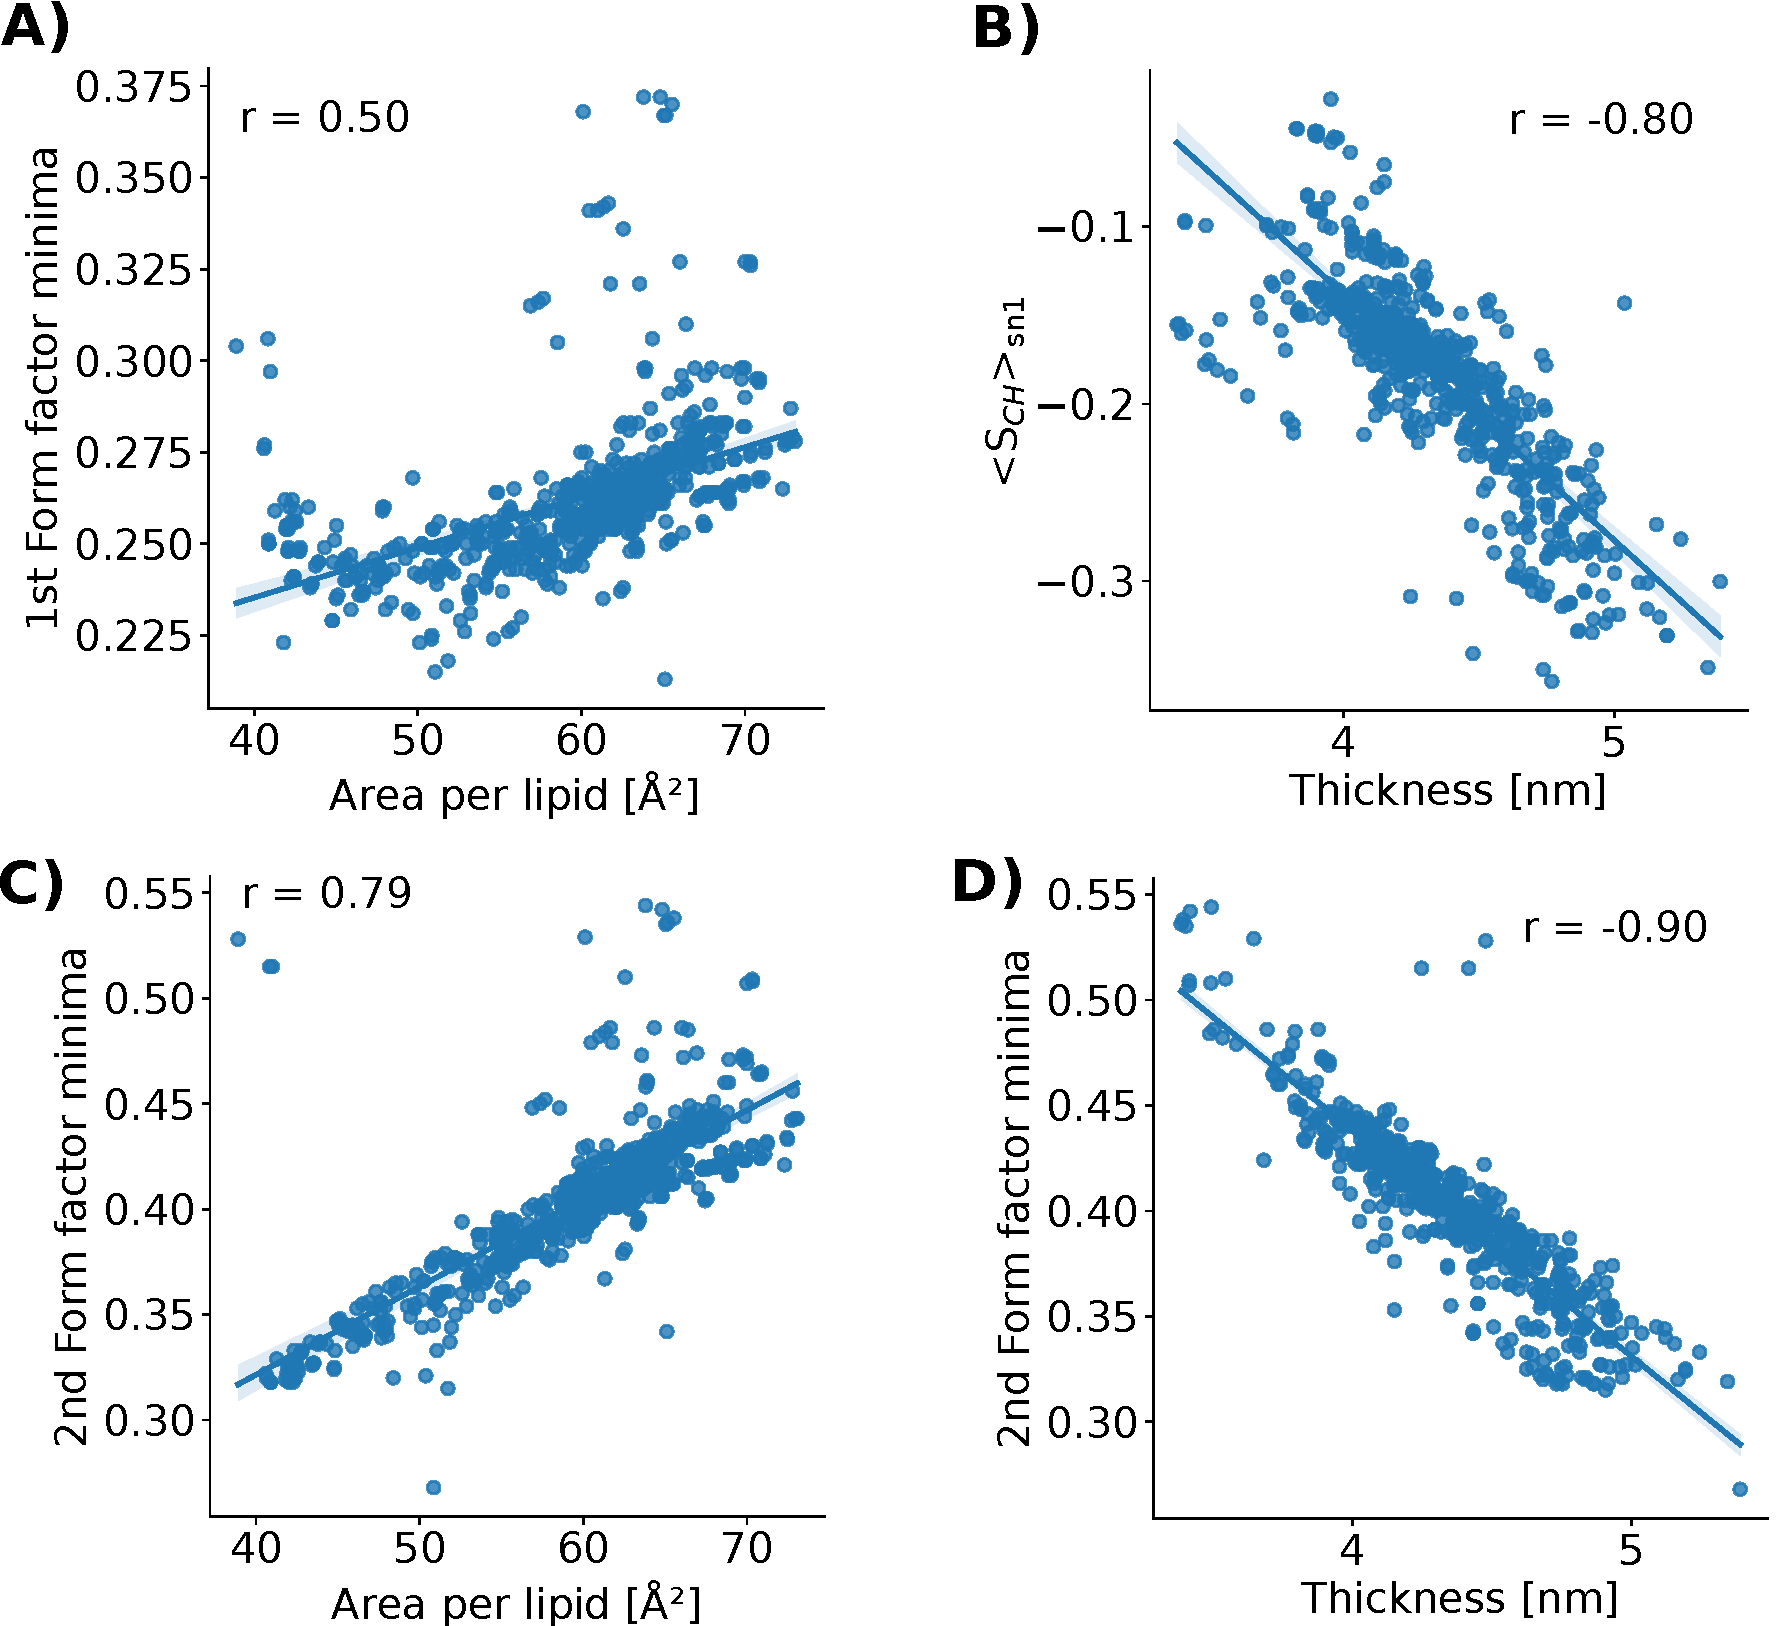
\includegraphics[width = 180mm]{Figures/QualityCorrelationsSI.pdf}
    \caption{Scatter plots and Pearson correlation coefficients, $r$, for the membrane area per lipid with X-ray scattering form factor minima (A and B), and for thickness with the average order parameter of the {\textit sn}-1 acyl chain (B) and with the second minimum from X-ray scattering form factors (D) extracted from the NMRlipids databank. All correlation coefficients have p-value below 0.001.}
    \label{fig:QualityCorrelationsSI}
\end{figure}


\pagebreak
\section{Dependence of form factor and order parameters on the simulation box size}

\begin{figure}[!h]
    \centerfloat
    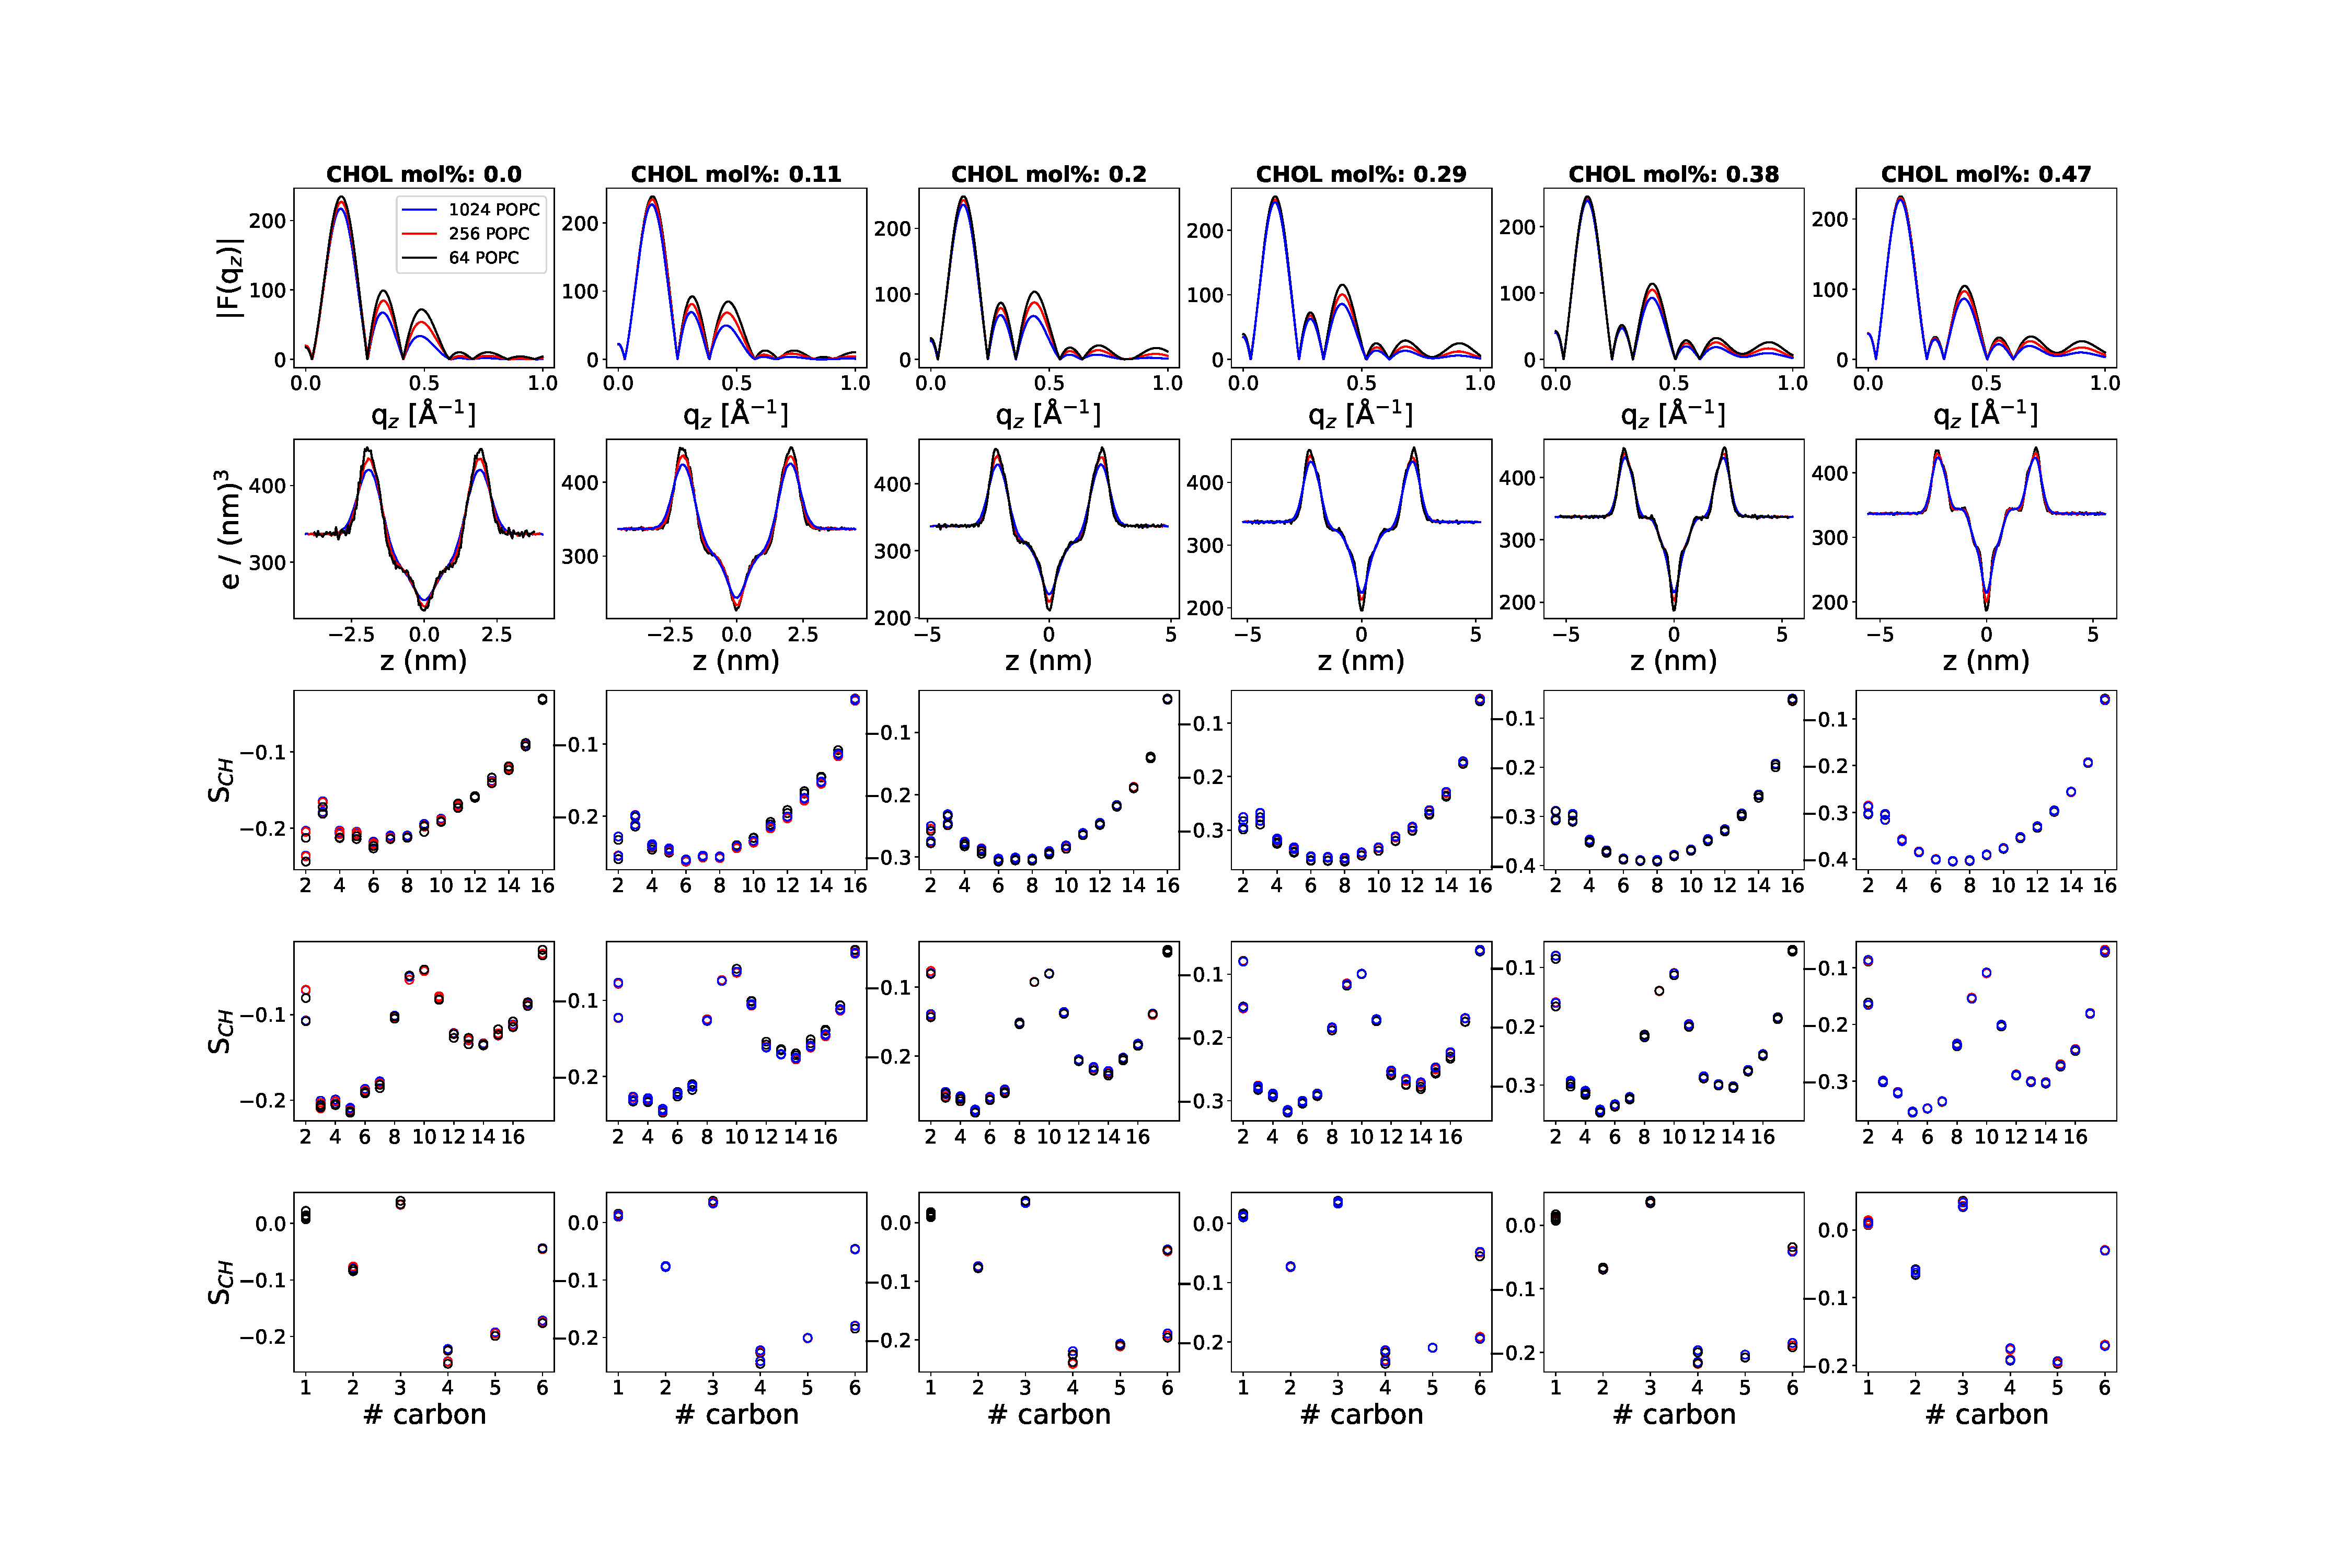
\includegraphics[width = 240mm]{Figures/SizeDependence.pdf}
    \caption{Dependence of the form factor $F(q_z)$, the electron density profiles along membrane normal, and the C--H bond order parameters $S_\mathrm{CH}$ (from top to bottom) on the simulation box size (with different columns showing different cholesterol concentrations). Simulations with 64, 256, and 1024 POPC lipids are from Ref.~\citenum{javanainen_matti_2021_7035350}. }
    \label{fig:sizedependence}
\end{figure}


\pagebreak
\section{Finding the best models for PC and PE mixtures}

\begin{figure}[!h]
    \centering
    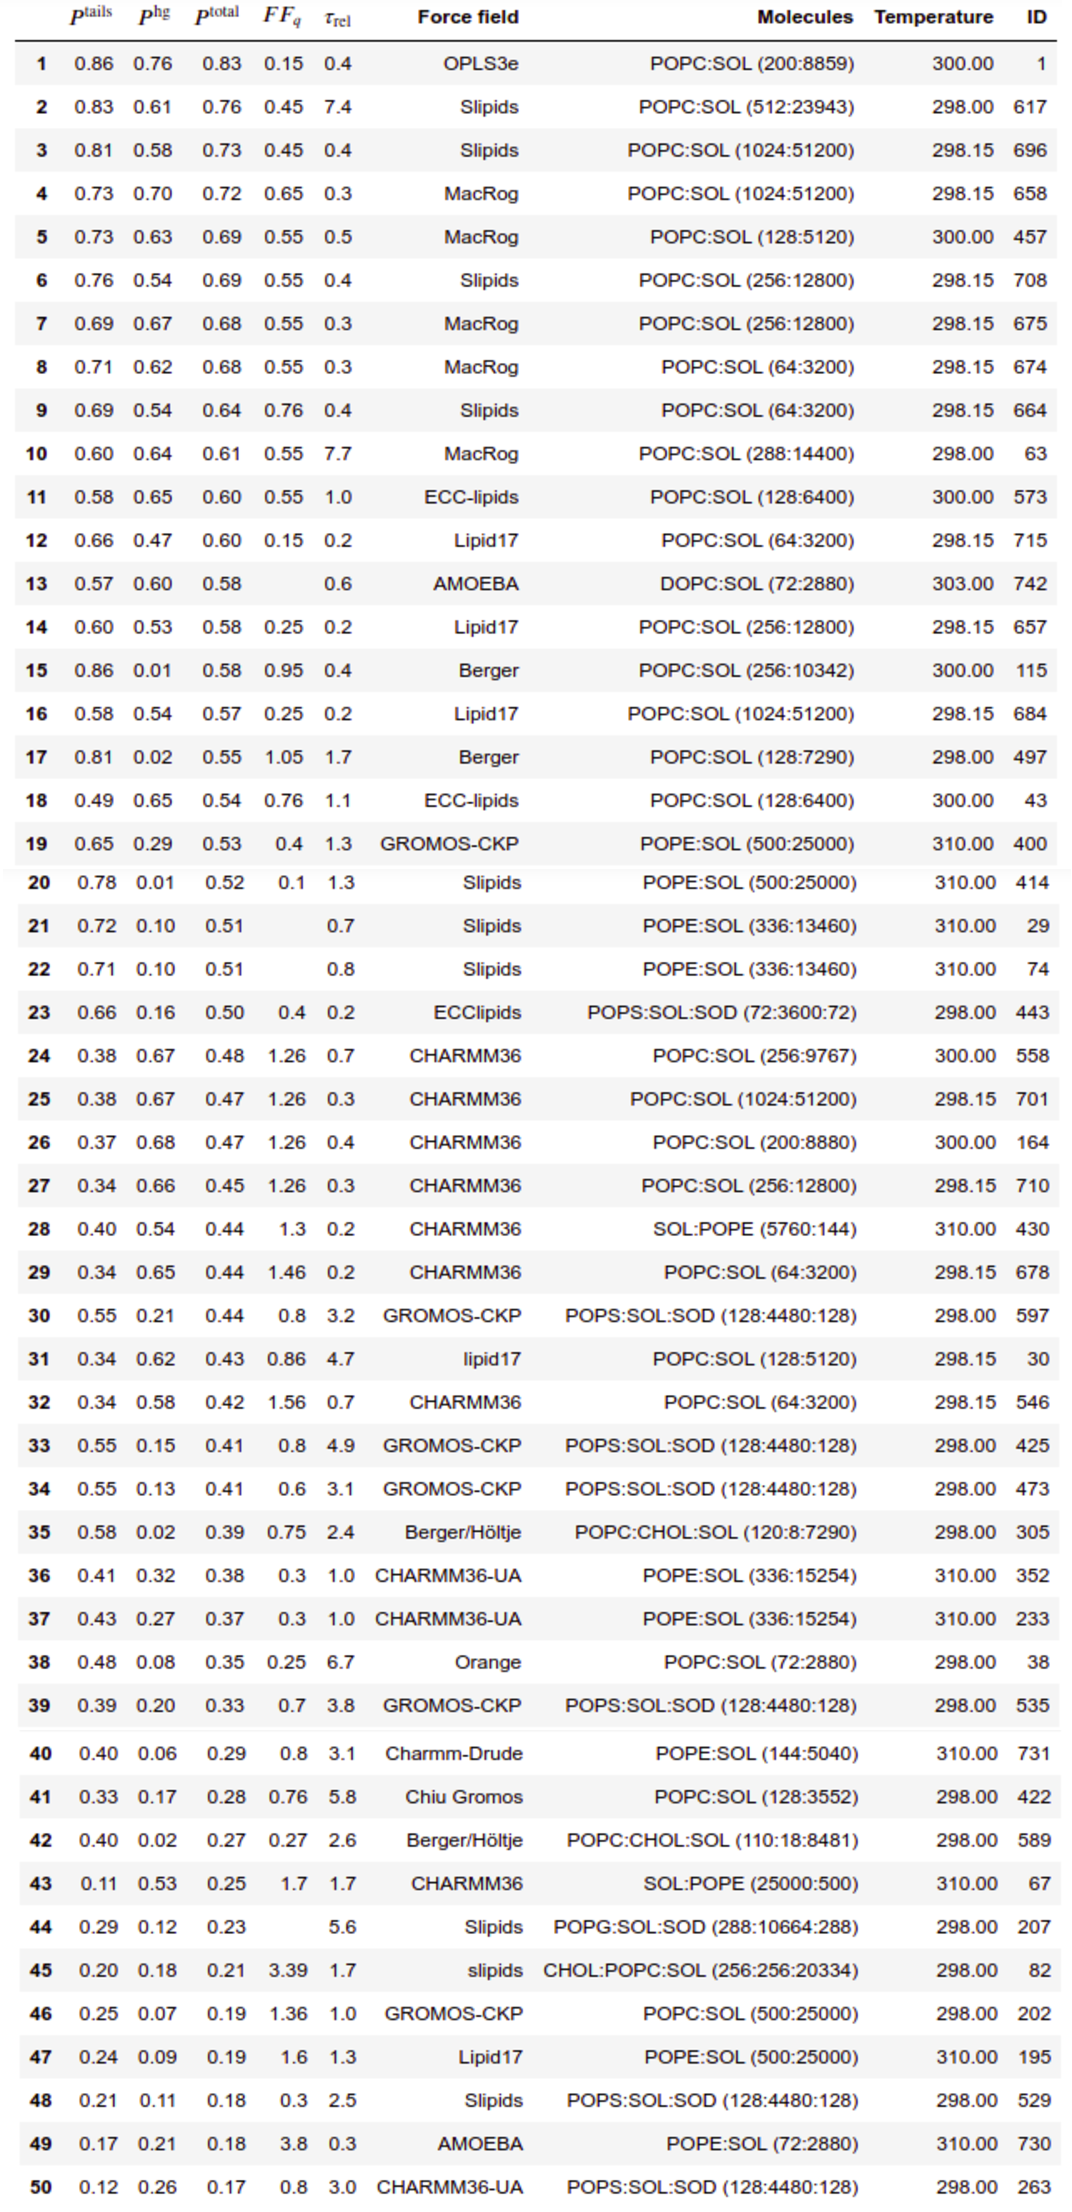
\includegraphics[height = 0.8\textheight]{Figures/totalrankingCOMPL.pdf}
    \caption{Top 50 simulations in the NMRlipids Databank ranked based on the C--H bond order parameter quality against experiments. The columns 2-4 show qualities for acyl chain order parameters ($P^\mathrm{tails}$), headgroup order parameters ($P^\mathrm{hg}$), all order parameters ($P^\mathrm{total}$), and for X-ray scattering form factors ($FF_q$). Column 5 shows relative equilibration times for conformations ($\tau_\mathrm{rel}$). Note that the best possible order parameter quality is one, while the best possible form factor quality is zero. ID values in the last column can be used to identify each simulation in the databank.}
    \label{fig:top50simulations}
\end{figure}


\begin{figure}[!h]
    \centering
    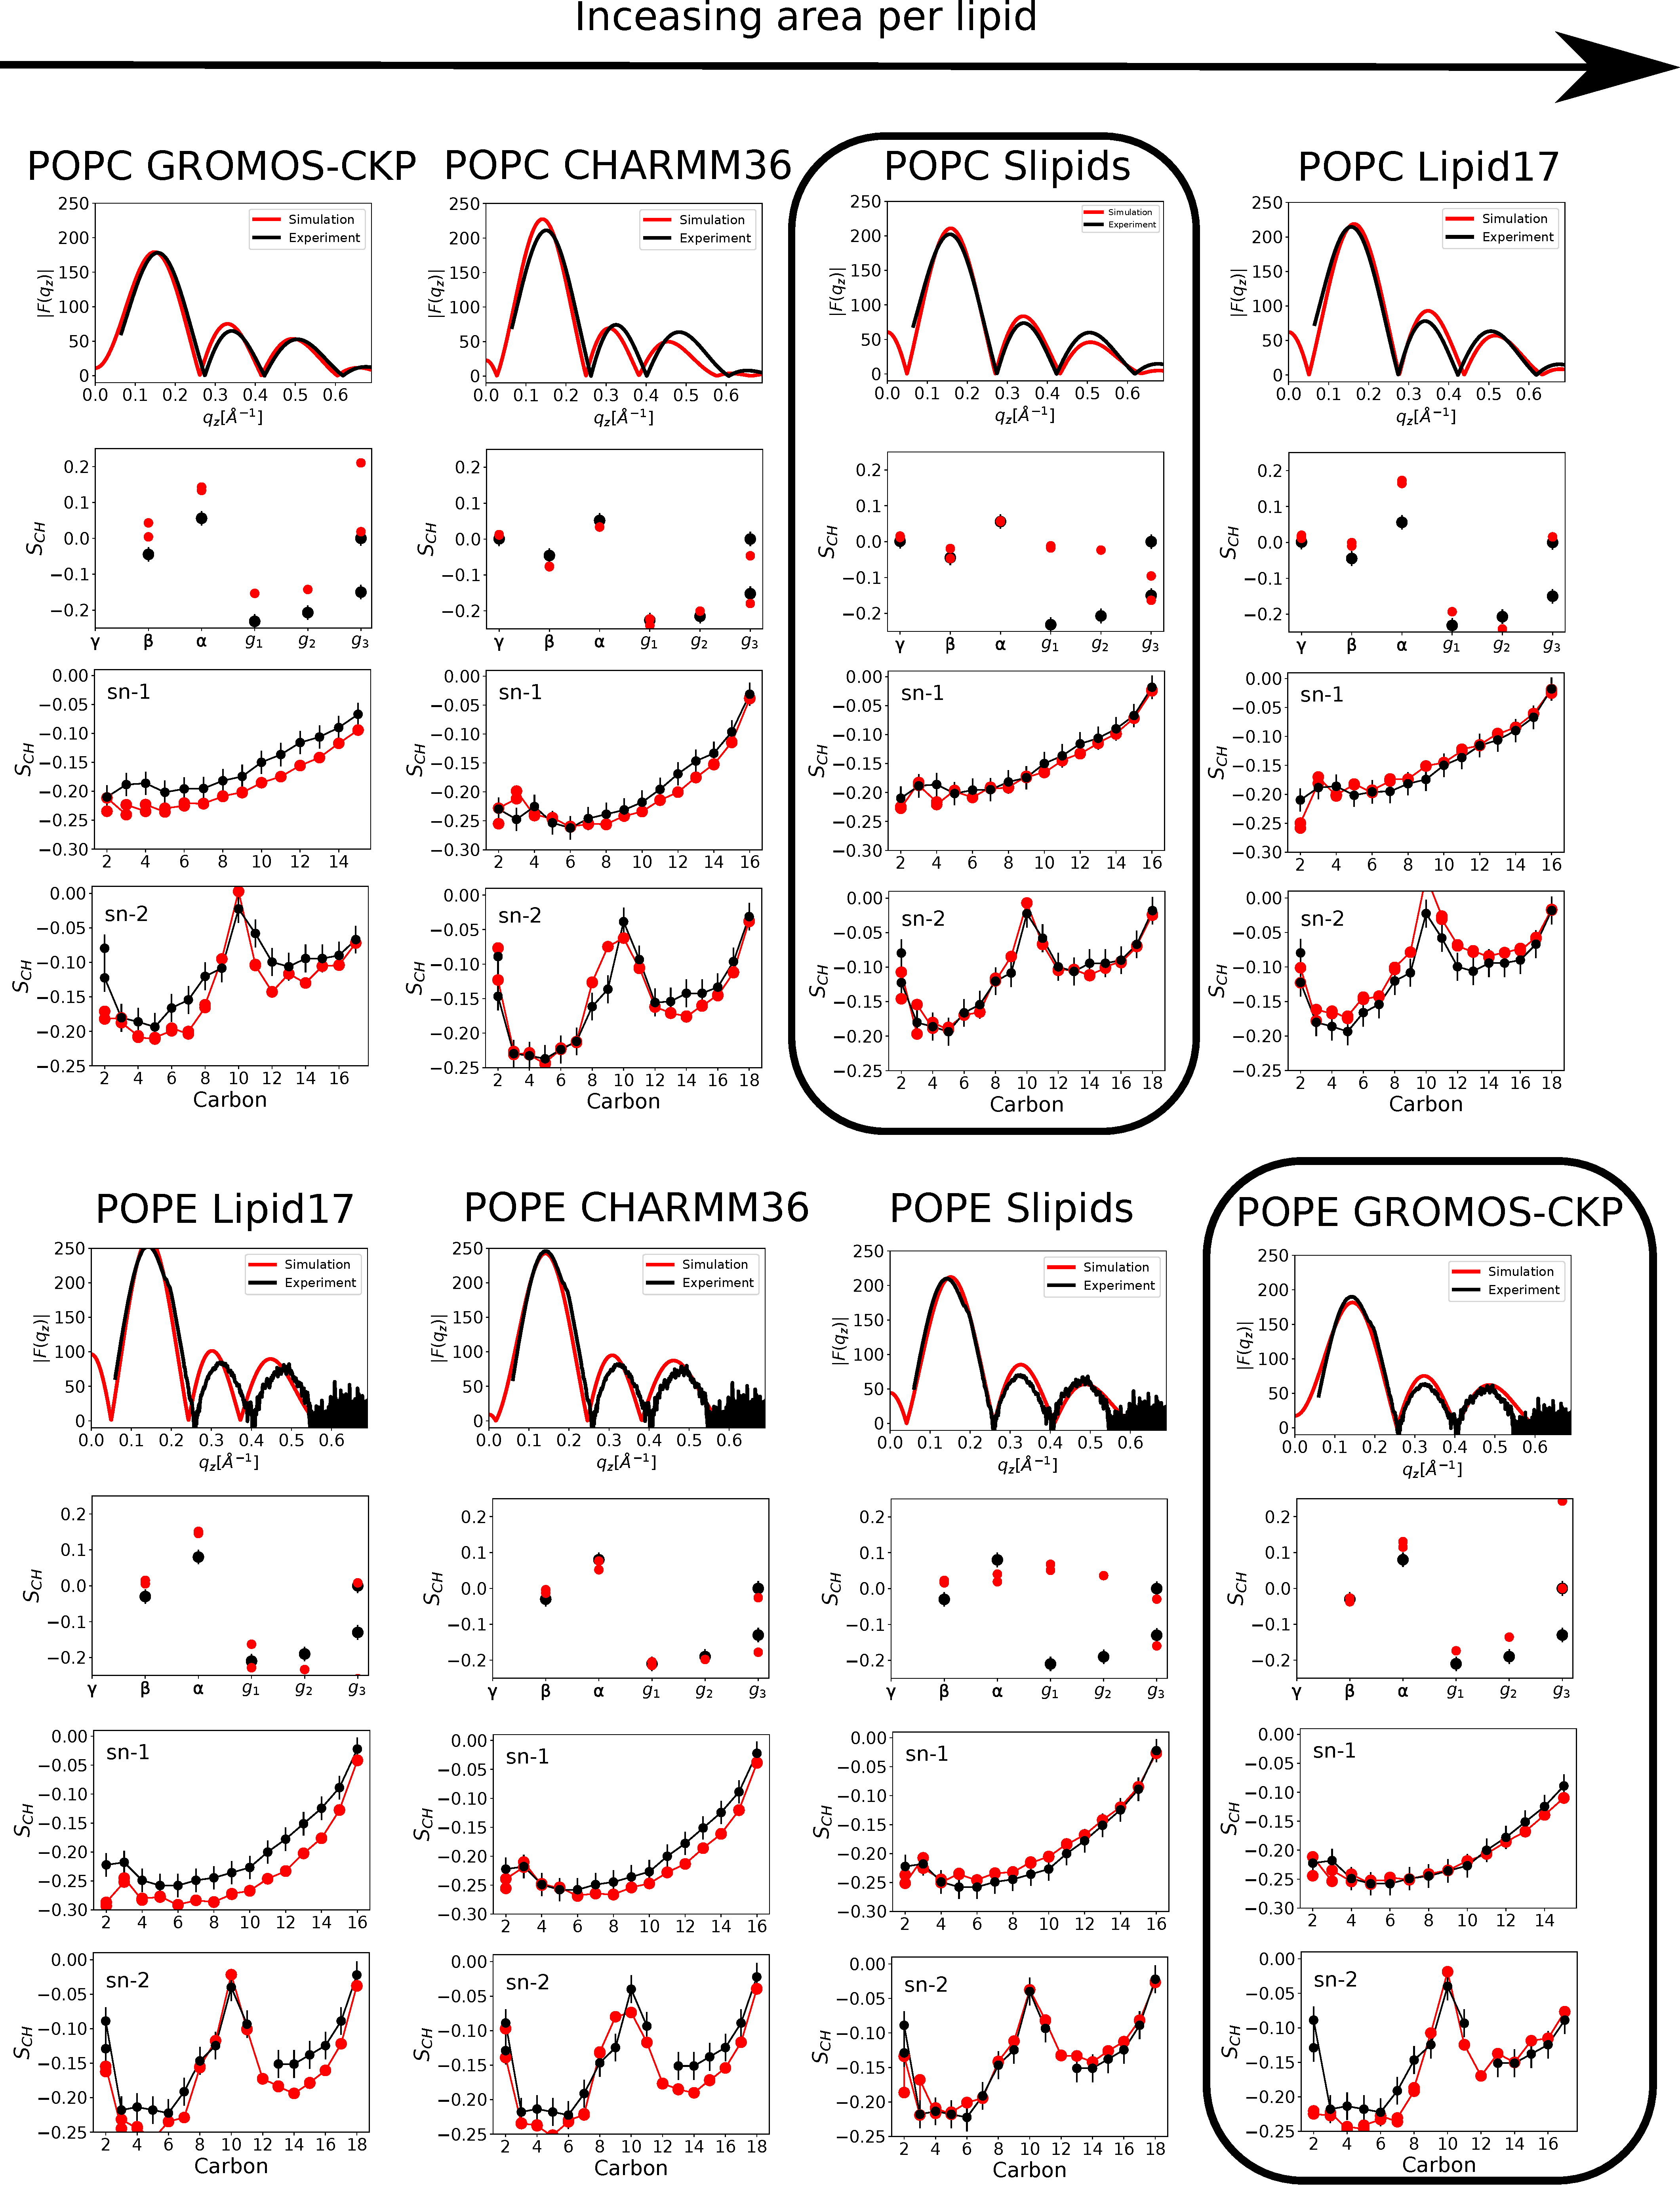
\includegraphics[height = 0.9\textheight]{Figures/POPC_POPE_dataSI.pdf}
    \caption{Simulations with the data for both POPC (top) and POPE (bottom) directly compared with the experimental data. The area per lipid increases from left to right. Simulations with the best overall quality for POPC and POPE order parameters are highlighted with a solid border.
  }
    \label{fig:POPC_POPE_dataSI}
\end{figure}


\pagebreak
\section{Water permeation through membranes}

\begin{figure}[!h]
    \centering
    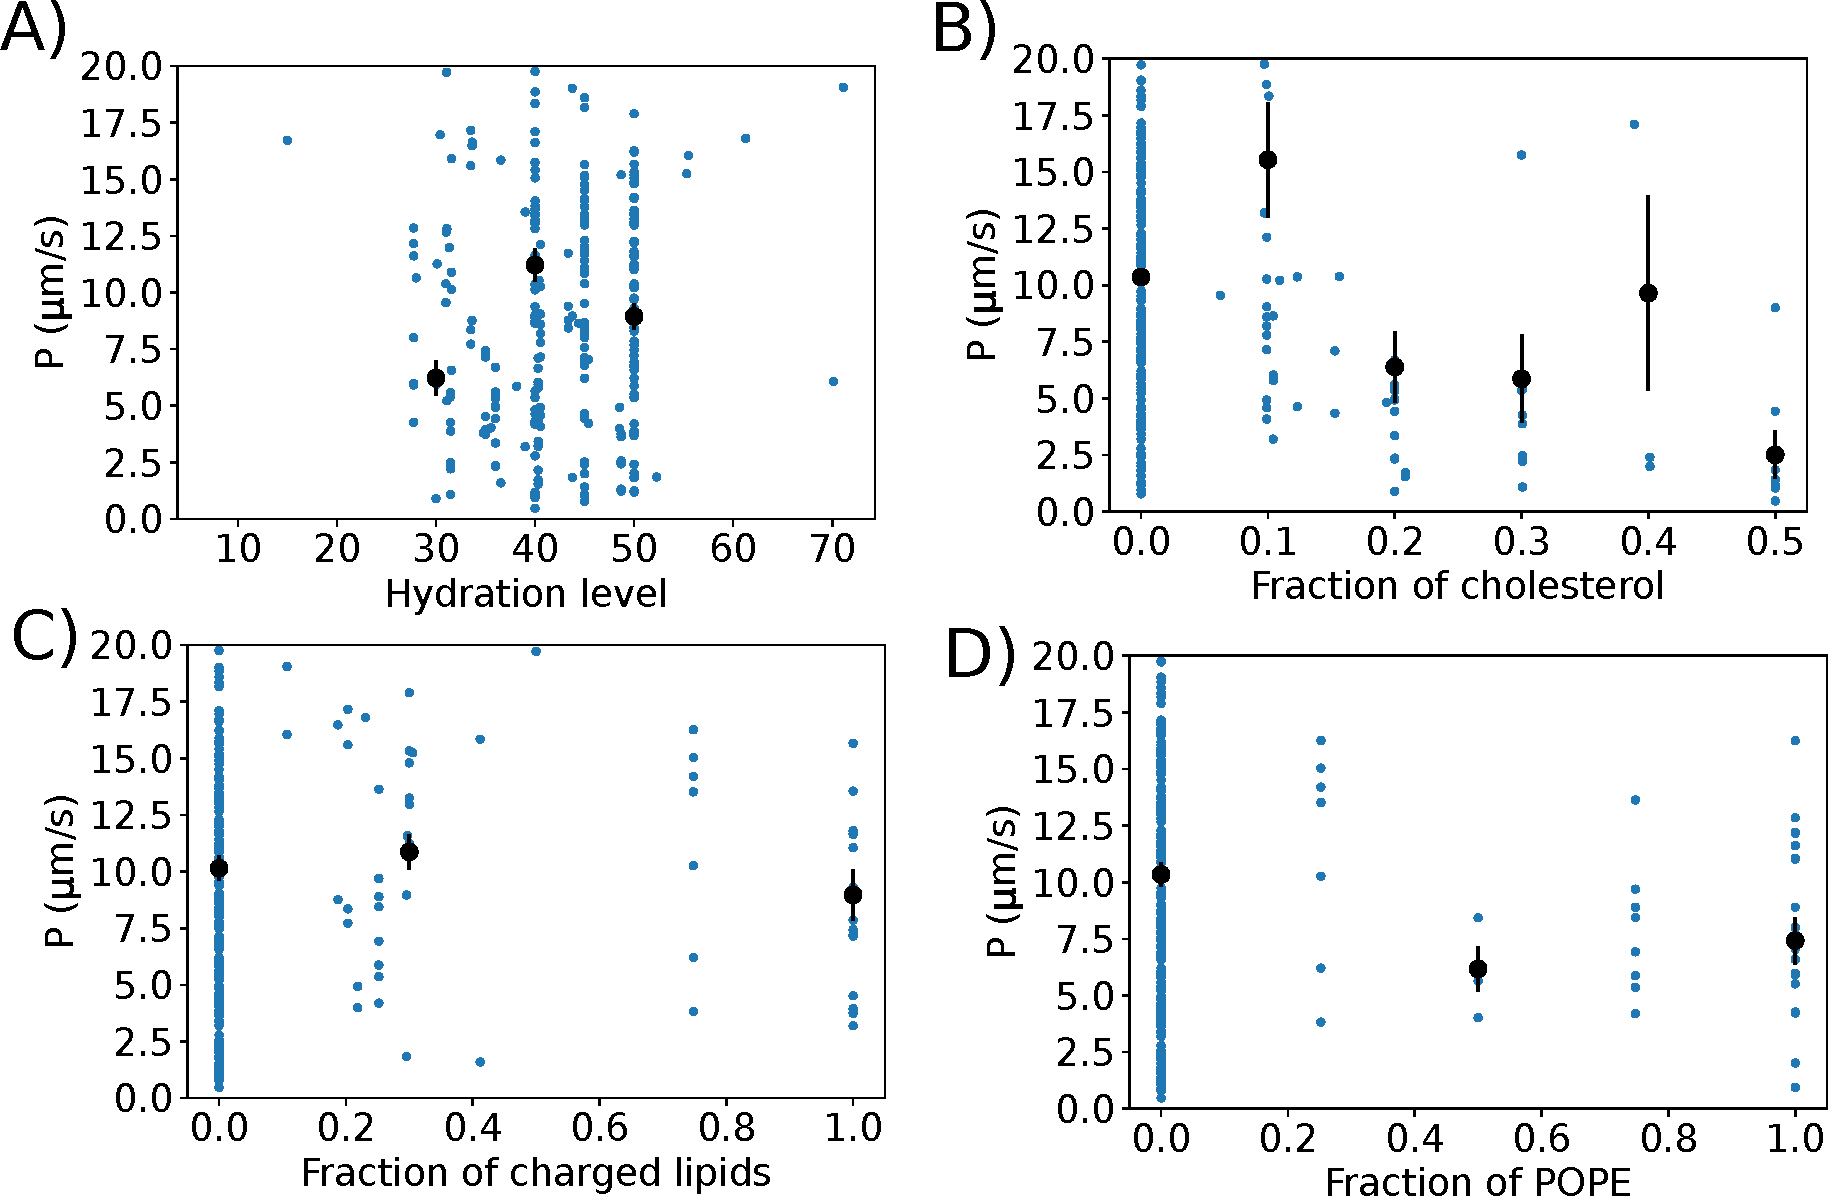
\includegraphics[width = \textwidth]{Figures/permeationSI.pdf}
    \caption{Water permeation through membranes analyzed from the Databank as a function of (A) hydration level, (B) fraction of cholesterol, (C) fraction of charged lipids, and (D) fraction of POPE in membrane. Values from simulations with non-zero permeation values are shown with blue dots. Histogrammed values are shown with black dots For the mean value in each bin, average weighted with the simulation lengths was used, and error bars show the standard error of the mean. Only bins with more than one microsecond of data were used. Only simulations with the temperatures between 300-315\,K were used.
    }
    \label{fig:permeationSI}
\end{figure}

\pagebreak
\section{Water diffusion along membranes}

\begin{figure}[!h]
    \centering
    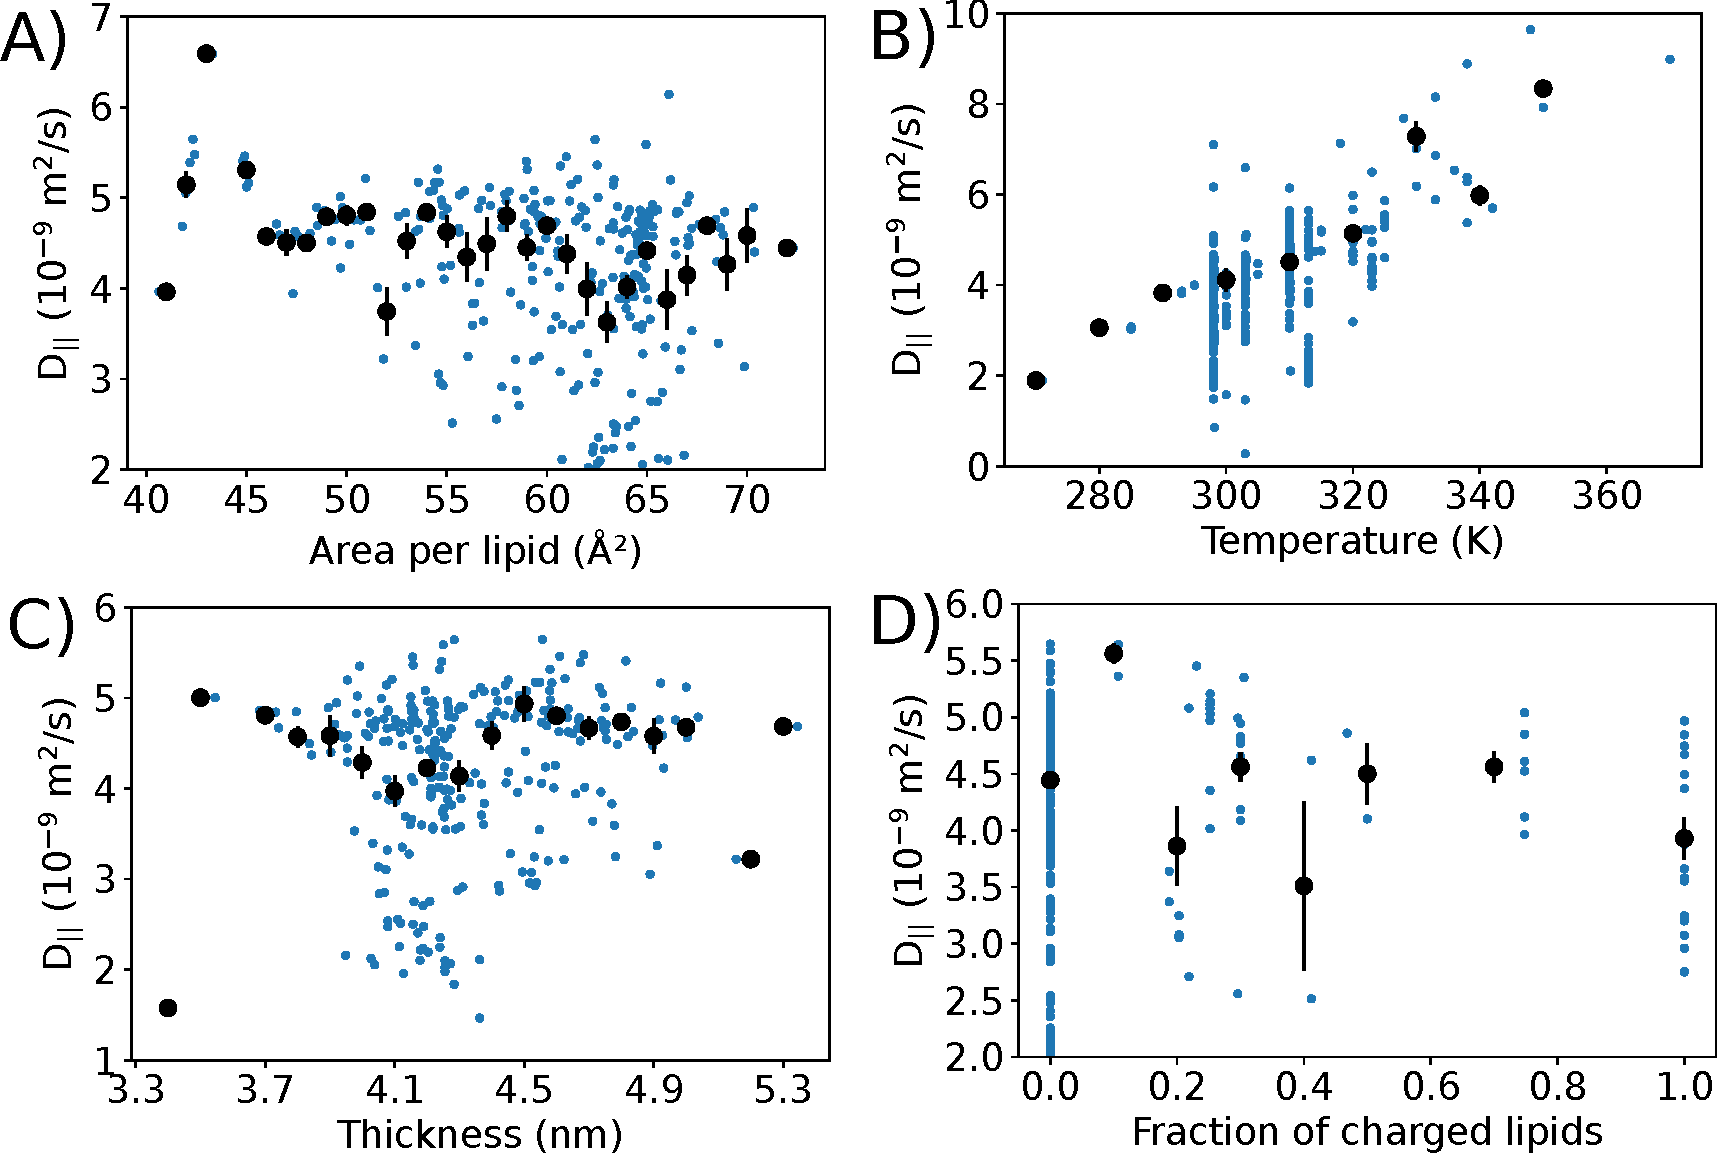
\includegraphics[width = \textwidth]{Figures/LateralDiffusionSI.pdf}
    \caption{Lateral diffusion of water as a function of (A) area per lipid, (B) temperature, (C) membrane thickness, and (D) fraction of charged lipids in a membrane. Non-zero permeation and diffusion values from simulations are shown with blue dots. Histogrammed values are shown with black dots. For the mean value in each bin, average weighted with the simulation lengths was used, and error bars show the standard error of the mean. Only bins with more than one microsecond of data in total were used for water permeation. Only simulations with the temperatures between 300-315\,K were used in D.}
    \label{fig:diffusionSI}
\end{figure}

%\newpage
\pagebreak
\section{Databank content}


\begin{figure}[!h]
  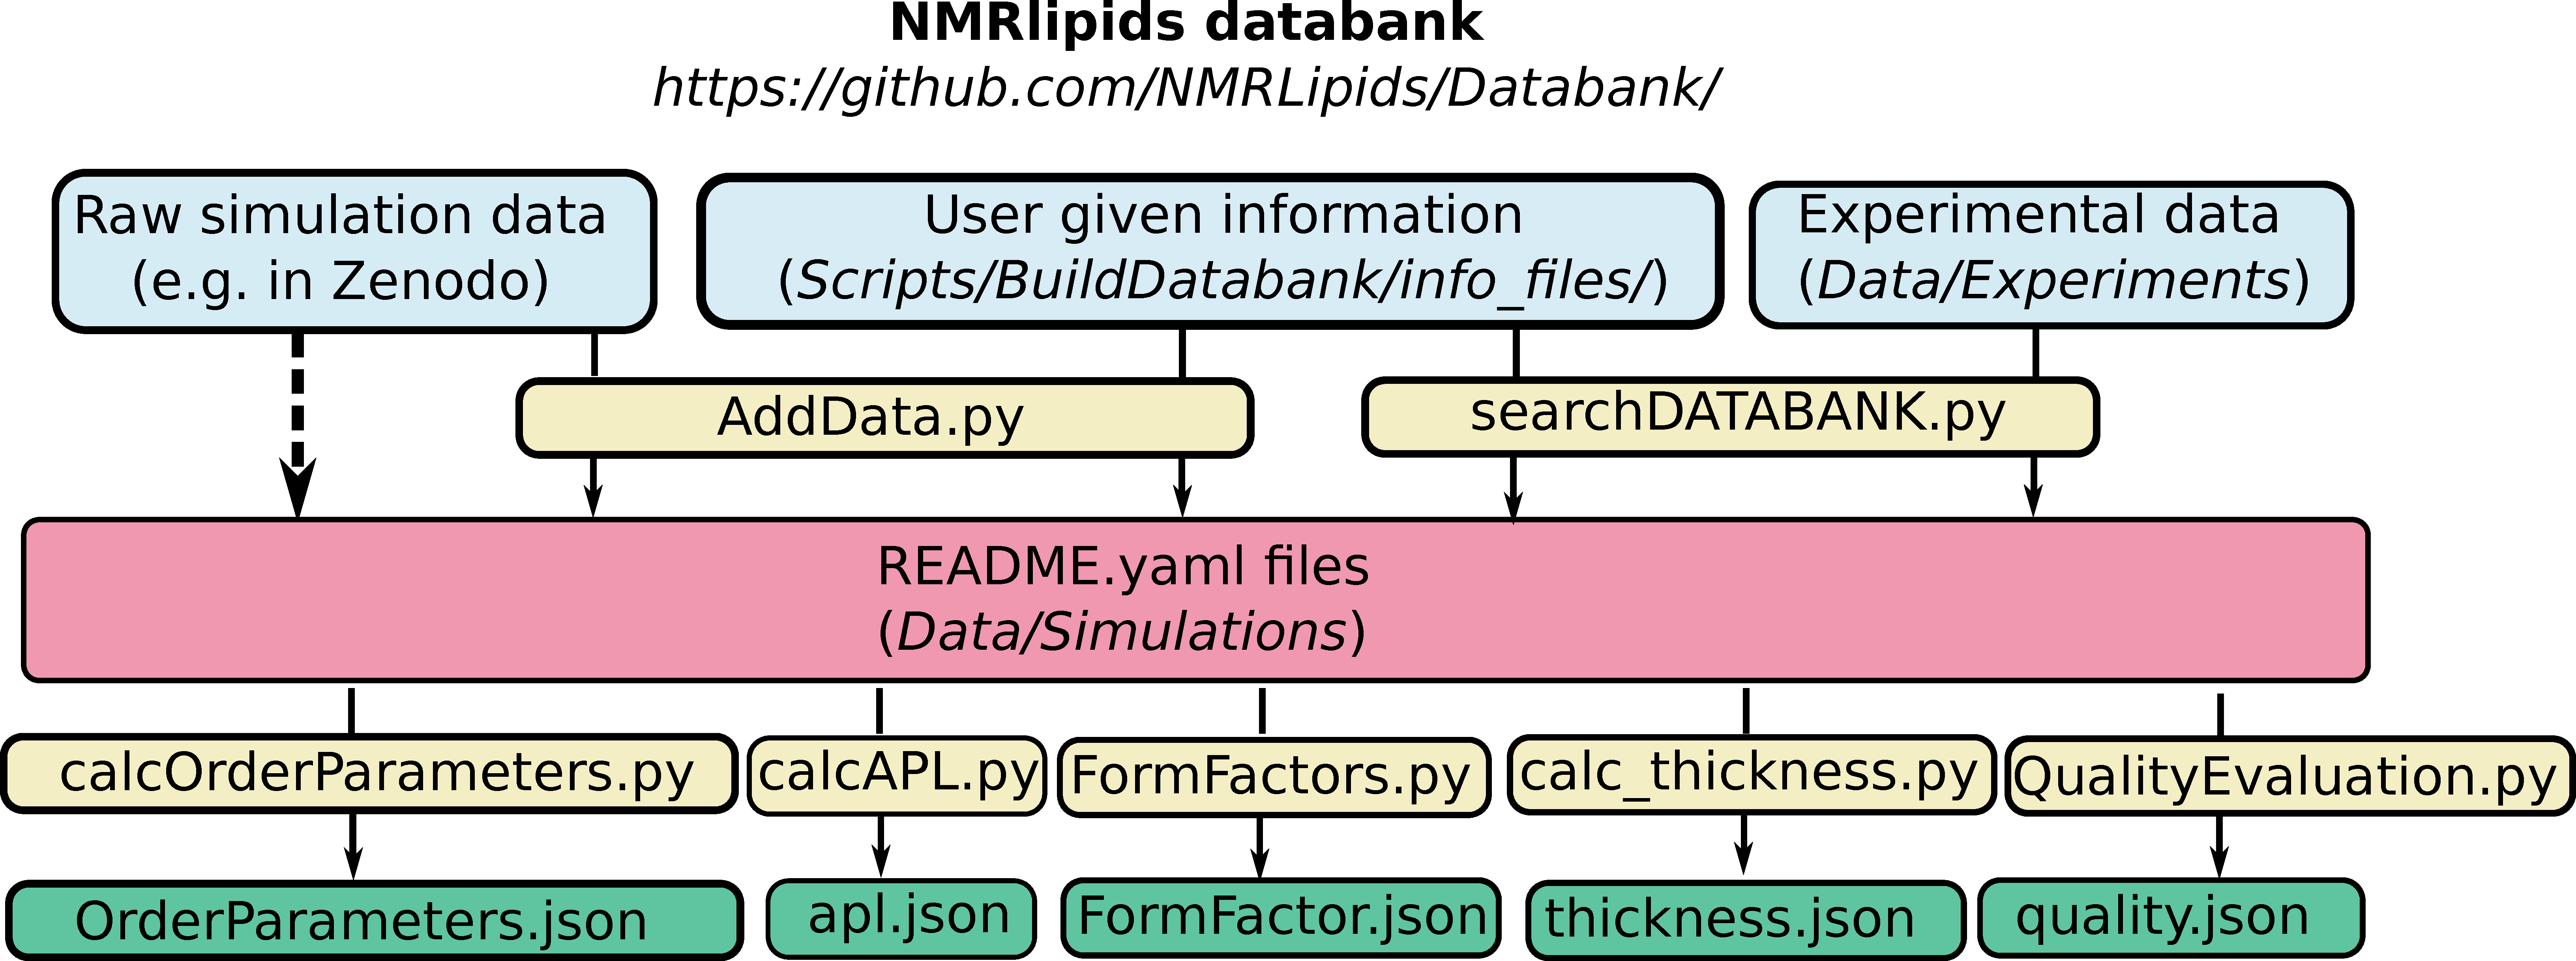
\includegraphics[width=\textwidth]{Figures/DataBankChart.pdf}
  \caption{Structure of the NMRlipids Databank. Manually added input data (blue boxes) include basic information on the simulation, permanent links to the raw data, and experimental data if available. The databank entries (red box) and analysis results (green boxes), at \url{https://github.com/NMRlipids/Databank/tree/main/Data/Simulations} are automatically generated by the computer programs included in the NMRlipids Databank (yellow boxes). Because the raw data are not permanently stored but can be accessed based on the information in the Databank, this connection is marked with a dashed line.}
  \label{DatabankStructure}
\end{figure}

\begin{table}[!h]
    \centering
    %\begin{tabular}{c c c c}
    \begin{tabular}{p{3.0cm}  p{5.0cm}  p{3.0cm}  p{4.0cm}}
        Code & Function & Input & Output \\
        \hline
        \multicolumn{4}{c}{ {\bf Databank layer}}\\
        \hline
        \multicolumn{4}{c}{ {\bf Scripts/BuildDatabank/ }}\\
         AddData.py & Create README.yaml from user given information in info.yaml  & info.yaml & README.yaml \\
         searchDATABANK.py & Pair simulations with available experimental data  & README.yaml files & Updated README.yaml files \\
         QualityEvaluation.py & Quality-evaluate simulations that are paired with experimental data  & README.yaml files & [lipid\_name]\_OrderParameters\_quality.json, [lipid\_name]\_FragmentQuality.json, system\_quality.json, FormFactorQuality.json \\
         \multicolumn{4}{c}{ {\bf Scripts/AnalyzeDatabank/ }}\\
         calcOrderParameters.py & Calculate C-H bond order parameters for all lipids in the simulation & README.yaml files & [lipid\_name]\_OrderParameters.json \\
         calcAPL.py & Calculate area per lipid as a function of time & README.yaml files & apl.json \\
         calc\_FormFactors.py & Calculate x-ray scattering form factors & README.yaml files & FormFactor.json \\
         calc\_thickness.py & Calculate membrane thickness & README.yaml files & thickness.json \\
         %template.py $\qquad$  template.ipynb & Minimal code to loop over simulations that can be used as a template for new analyses & README.yaml files & \\
         
    \end{tabular}
    \caption{List of relevant codes used to build the Databank and perform analyses in the {\it Databank layer} available at~\url{https://github.com/NMRLipids/Databank/}.}
    \label{tab:codes}
\end{table}

\begin{table}[!h]
    \centering
    %\begin{tabular}{c c c c}
    \begin{tabular}{p{3.5cm}  p{4.5cm}  p{3.0cm}  p{4.0cm}}
        Code & Function & Input & Output \\
        \hline
        \multicolumn{4}{c}{ {\bf Application layer}}\\
        \hline
        %\multicolumn{4}{c}{ {\bf Scripts/BuildDatabank/ }}\\
        AreaPerLipidAnd ThicknessCorrelations.ipynb  & Analyze correlations between results in the {\it Databank layer}  & Results in the {\it Databank layer} & Figs.~\ref{fig:quality}G and~\ref{fig:QualityCorrelationsSI} \\
        FlipFlop.py & Calculate flip-flop rates of lipids in all simulations & README.yaml & flipflop.dat files at {\it /Data/Flipflops/} \\
        plotFlipFlop.ipynb & Plot how flip-flop rates depend on membrane properties & README.yaml and flipflop.dat files at {\it /Data/Flipflops/} & Fig.~\ref{fig:flip-flops} \\
        calcMD-PERMEATION.py  & Calculate permeation rate of water molecules through bilayers from all simulations & README.yaml & Counting\_events.txt files at {\it /Data/MD-PERMEATION/} \\
        calcWATERdiffusion.py & Calculate water lateral diffusion along membrane surface & README.yaml & WATERlateralMSD.xvg files at {\it /Data/WATERdiffusion/} \\
        plotWaterPermeation.ipynb & Plot how water permeation and diffusion depend on membrane properties & README.yaml, Counting\_events.txt\,at {\it /Data/MD-PERMEATION/} and\,WATERlateralMSD.xvg files\,at {\it /Data/WATERdiffusion/} & Figs.~\ref{fig:permeability},~\ref{fig:permeationSI}, and~\ref{fig:diffusionSI}. \\
        plotSimulation.ipynb & Plot results from a simulation together with the experimental data if available & README.yaml files and results in the {\it databank layer} & Figs~\ref{fig:quality}D-F and ~\ref{fig:POPC_POPE_dataSI}
    \end{tabular}
    \caption{Examples of codes that analyze membrane properties from the Databank in an {\it Application layer} available at~\url{https://github.com/NMRLipids/DataBankManuscript/}.}
    \label{tab:codesApplication}
\end{table}


\begin{table}[p]
    \centering
    \begin{tabular}{  p{3.5cm}  p{9.5cm}  p{4.0cm} }
    \toprule
    key & description & type  \\
    \midrule
        %\hline
    DOI & DOI from where the raw data is found & user given (compulsory) \\
    SOFTWARE & Software used to run the simulation (Gromacs, Amber, NAMD, etc.) & \\
    TRJ & Name of the trajectory file found from DOI (trr or xtc for Gromacs, dcd for OpenMM) & \\
    TPR (Gromacs) & Name of the tpr topology file found from DOI for Gromacs simulations & \\
    PDB (OpenMM) & Name of the pdb file found from DOI for OpenMM simulations & \\
    PREEQTIME & Pre-equilibrate time simulated before the uploaded trajectory in nanoseconds. 
    %For example, if you upload 100-200 ns part of total 200 ns simulation, this should value should be 100. 
    & \\
    TIMELEFTOUT & Equilibration period in the uploaded trajectory that should be discarded in analyses. 
    %For example, if you upload 0-200 ns part of total 200 ns simulation where the first 100 ns should be considered as an equilibration, this value should be 100. 
    & \\
    COMPOSITION & Dictionary connecting universal molecule and atom names to the ones used in simulation & \\
    DIR\_WRK & Temporary working directory in your local computer. \\
    UNITEDATOM\_DICT & Information for constucting hydrogens for united atom simulations using buildH program~\cite{santuz21}. Empty for all atom simulations. & \\
    TYPEOFSYSTEM & Lipid bilayer or something else & \\
    \hline
    PUBLICATION & Give reference to a publication(s) related to the data & user given (optional)\\
    AUTHORS\_CONTACT & Name and email of the main author(s) of the data & \\
    SYSTEM & System description on free text format & \\
    SOFTWARE\_VERSION & Version of the used software & \\
    FF & Name of the used force field & \\
    FF\_SOURCE & Source of the force field parameters, e.g, CHARMM-GUI, webpage, citation to a publication & \\
    FF\_DATE &  Date when force field parameters were accessed on the given source (day/month/year) & \\
    FF{molename} & Molecule specific force field information, e.g., water model with FFSOL and sodium parameters with FFSOD & \\
    CPT & Name of the Gromacs checkpoint file & \\
    LOG & Name of the Gromacs log file & \\
    GRO & Name of the Gromacs gro file & \\
    TOP & Name of top file for Gromacs or psf file for OpenMM & \\
    CRD & Name of crd file for OpenMM & \\
    WARNINGS & Dictionary containing information about unusual features in the trajectory, such as ambiguous atom names, membrane normal not oriented in $z$-direction, old Gromacs version used & \\
    \hline
    TRAJECTORY\_SIZE & Size of the trajectory file in bytes & automatically extracted data \\
    TRJLENGTH & Lenght of the trajectory (ps) & \\
    TEMPERATURE & Temperature of the simulation & \\
    NUMBER\_OF\_ATOMS & Number of atoms in the simulation & \\
    DATEOFRUNNIG & Date when added into the Databank & \\
    EXPERIMENT & Potentially connected experimental data & \\
    COMPOSITION & Numbers of lipid molecules in both leaflets and numbers of other molecules are added to the dictionary & \\
    ID & Unique ID number to ease the analyses & \\
    \end{tabular}
    \caption{Keys stored in the README.yaml files of simulations.}
    \label{tab:READMEkeys}
\end{table}

%\begin{table}[h]
%    \centering
%    \begin{tabular}{c|c}
%        Abbreviation & Molecule name \\
%        \hline
%        POPC &  1-palmitoyl-2-oleoyl-sn-glycero-3-phosphocholine\\
%        POPG &  1-palmitoyl-2-oleoyl-sn-glycero-3-phosphoglycerol \\
%        POPS & 1-palmitoyl-2-oleoyl-sn-glycero-3-phospho-L-serine \\
%        POPE & 1-palmitoyl-2-oleoyl-sn-glycero-3-phosphoethanolamine \\
%        CHOL & cholesterol \\
%        DHMDMAB & dihexadecyldimethylammonium \\
%        \hline
%        POT & potassium ion \\
%%        SOD & sodium ion \\
 %       CLA & chloride ion \\
%        CAL & calcium ion \\
%%    \end{tabular}
 %   \caption{Abbreviations used in the databank}
%    \label{tab:abbreviations}
%\end{table}


\begin{table}[h]
    \centering
    \begin{tabular}{  p{5.0cm}  p{10.0cm}}
    \toprule
    key & description \\
    \midrule
    DOI & DOI of the publication related to the experimental data \\
    TEMPERATURE & Temperature of the experiment \\
    MOLAR\_FRACTIONS & Dictionary of molar fractions of bilayer components \\
    ION\_CONCENTRATIONS & Dictionary of ion concentrations of the system \\
    % (defined as ??) \\
    TOTAL\_LIPID\_CONCENTRATION & Total concentration of lipid components; if exact concentration is not known, but experiments are performed in excess water, 'full hydration' can be given \\
    COUNTER\_IONS & Type of counter ions if present
\end{tabular}
    \caption{Keys stored in the README.yaml files of experiments.}
    \label{tab:READMEkeysEXP}
\end{table}

\begin{comment}
    

\begin{table}[p]
    \centering
    \begin{tabular}{c c}
    Abbreviation & Molecule name \\
    \hline
    Lipids and surfactants & \\
    \hline
    POPC &  1-palmitoyl-2-oleoyl-sn-glycero-3-phosphocholine  \\
    POPG &  1-palmitoyl-2-oleoyl-sn-glycero-3-phosphoglycerol \\
    POPS & 1-palmitoyl-2-oleoyl-sn-glycero-3-phospho-L-serine \\
    POPE & 1-palmitoyl-2-oleoyl-sn-glycero-3-phosphoethanolamine \\
    PYPC & 1-(16:0)-2-(16:1$^\Delta9$)-sn-glycero-3-phosphocholine \\
    PAzePCprot & 1-palmitoyl-2-azelaoyl-sn-glycero-3-phosphocholine protonated \\
    PAzePCdeprot & 1-palmitoyl-2-azelaoyl-sn-glycero-3-phosphocholine deprotonated \\
    DMPC & 1,2-dimyristoyl-sn-glycero-3-phosphocholine \\
    DPPC & 1,2-dipalmitoyl-sn-glycero-3-phosphocholine \\
    DPPE & 1,2-dipalmitoyl-sn-glycero-3-phosphoethanolamine \\
    DPPG & 1,2-dipalmitoyl-sn-glycero-3-phospho-(1'-rac-glycerol) (sodium salt) \\
    DEPC & 1,2-dierucoyl-sn-glycero-3-phosphocholine \\
    DRPC & 1,2-(14:1$^\Delta9$)-sn-glycero-3-phosphocholine \\
    DYPC & 1,2-(16:1$^\Delta9$)-sn-glycero-3-phosphocholine \\
    DLPC & 1,2-dilauroyl-sn-glycero-3-phosphocholine \\
    DLIPC& 1,2-dilinoleoyl-sn-glycero-3-phosphocholine \\
    DOG  & 1,2-dioleoyl-sn-glycerol \\
    DOPC & 1,2-dioleoyl-sn-glycero-3-phosphocholine \\
    DOPE & 1,2-dioleoyl-sn-glycero-3-phosphoethanolamine \\
    DDOPC& 1,2-didocosahexaenoyl-sn-glycero-3-phosphocholine \\
    DOPS & 1,2-dioleoyl-sn-glycero-3-phospho-L-serine \\
    DSPC & 1,2-distearoyl-sn-glycero-3-phosphocholine \\
    DAPC & 1,2-diarachidonoyl-sn-glycero-3-phosphocholine \\
    SLiPC & 1-(18:0)-2-(18:2 $^{\Delta9,12}$)-sn-glycero-3-phosphocholine  \\
    DMTAP & 1,2-dimyristoyl-3-trimethylammonium-propane \\
    SOPC & 1-stearoyl-2-oleoyl-sn-glycero-3-phosphocholine \\
    POPI & \\ 
    SAPI & \\
    SLPI &  \\
    SDG & 1-stearoyl-2-docosahexaenoyl-sn-glycerol \\
    SDPE & 1-stearoyl-2-docosahexaenoyl-sn-glycero-3-phosphoethanolamine \\
    CER  & N-palmitoyl-D-erythro-sphingosine \\
    CHOL & cholesterol  \\
    DCHOL & 18,19-di-nor-cholesterol \\
    DHMDMAB & dihexadecyldimethylammonium  \\
    \hline
    Other molecules & \\
    \hline
    POT & potassium ion  \\
    SOD & sodium ion  \\
    CLA & chloride ion \\
    CAL & calcium ion  \\
    CES & caesium ion \\
    SOL & water  \\
    \end{tabular}
    \caption{Abbreviations for molecule names used in the Databank.}
    \label{tab:abbreviations}
\end{table}
\end{comment}

\begin{table}[p]
    \centering
    \begin{tabular}{l}
    Force field name and references \\
    \hline
    CHARMM36~\cite{klauda10}\\
    Slipids~\cite{jambeck12,jambeck12b,jambeck2012another,ermilova16,grote20}  \\
    MacRog~\cite{Kulig15b}  \\
    Amber Lipid14/17~\cite{dickson14,dickson22}  \\
    Charmm-Drude~\cite{li2017drude}      \\
    ECClipids~\cite{melcr18,melcr20,bacle21}  \\
    GROMOS-CKP~\cite{Chandrasekhar03,kukol09,piggot12}  \\
    Berger~\cite{berger97}  \\
    ECC-CHARMM36~\cite{nencini2019development}  \\
    Orange~\cite{catte16}  \\
    Poger~\cite{poger10}  \\
    GROMOS 43A1-S3~\cite{chiu09}  \\ 
    GAFFlipid~\cite{dickson12}  \\
    OPLS3e~\cite{roos19}  \\
    Ulmschneider~\cite{Ulmschneider09}  \\
    Chiu Gromos~\cite{chiu09}  \\
    AMOEBA~\cite{chu2018polarizable} \\
    \end{tabular}
    \caption{List of current force fields used in simulations in the Databank, with references.}
    \label{tab:ForceFields}
\end{table}



\clearpage
%\section{Experimental data}
\section{NMR experiments}
Acyl chain order parameters of POPE (Figs.~\ref{POPEexp1} and~\ref{POPEexp2}) and POPG (Figs.~\ref{POPGexp1} and~\ref{POPGexp2}) were analyzed from the same data that were previously recorded to determine headgroup order parameters~\cite{bacle21}. The analysis of the crowded spectral region at 29--31 ppm was based on the previous assignment reported for POPC membranes~\cite{ferreira13}. To measure the order parameters for DOPC (Fig.~\ref{fig:DOPCexp}), the sample was prepared and experiments performed similarly to previous studies~\cite{bacle21}.

\begin{figure}[h]
  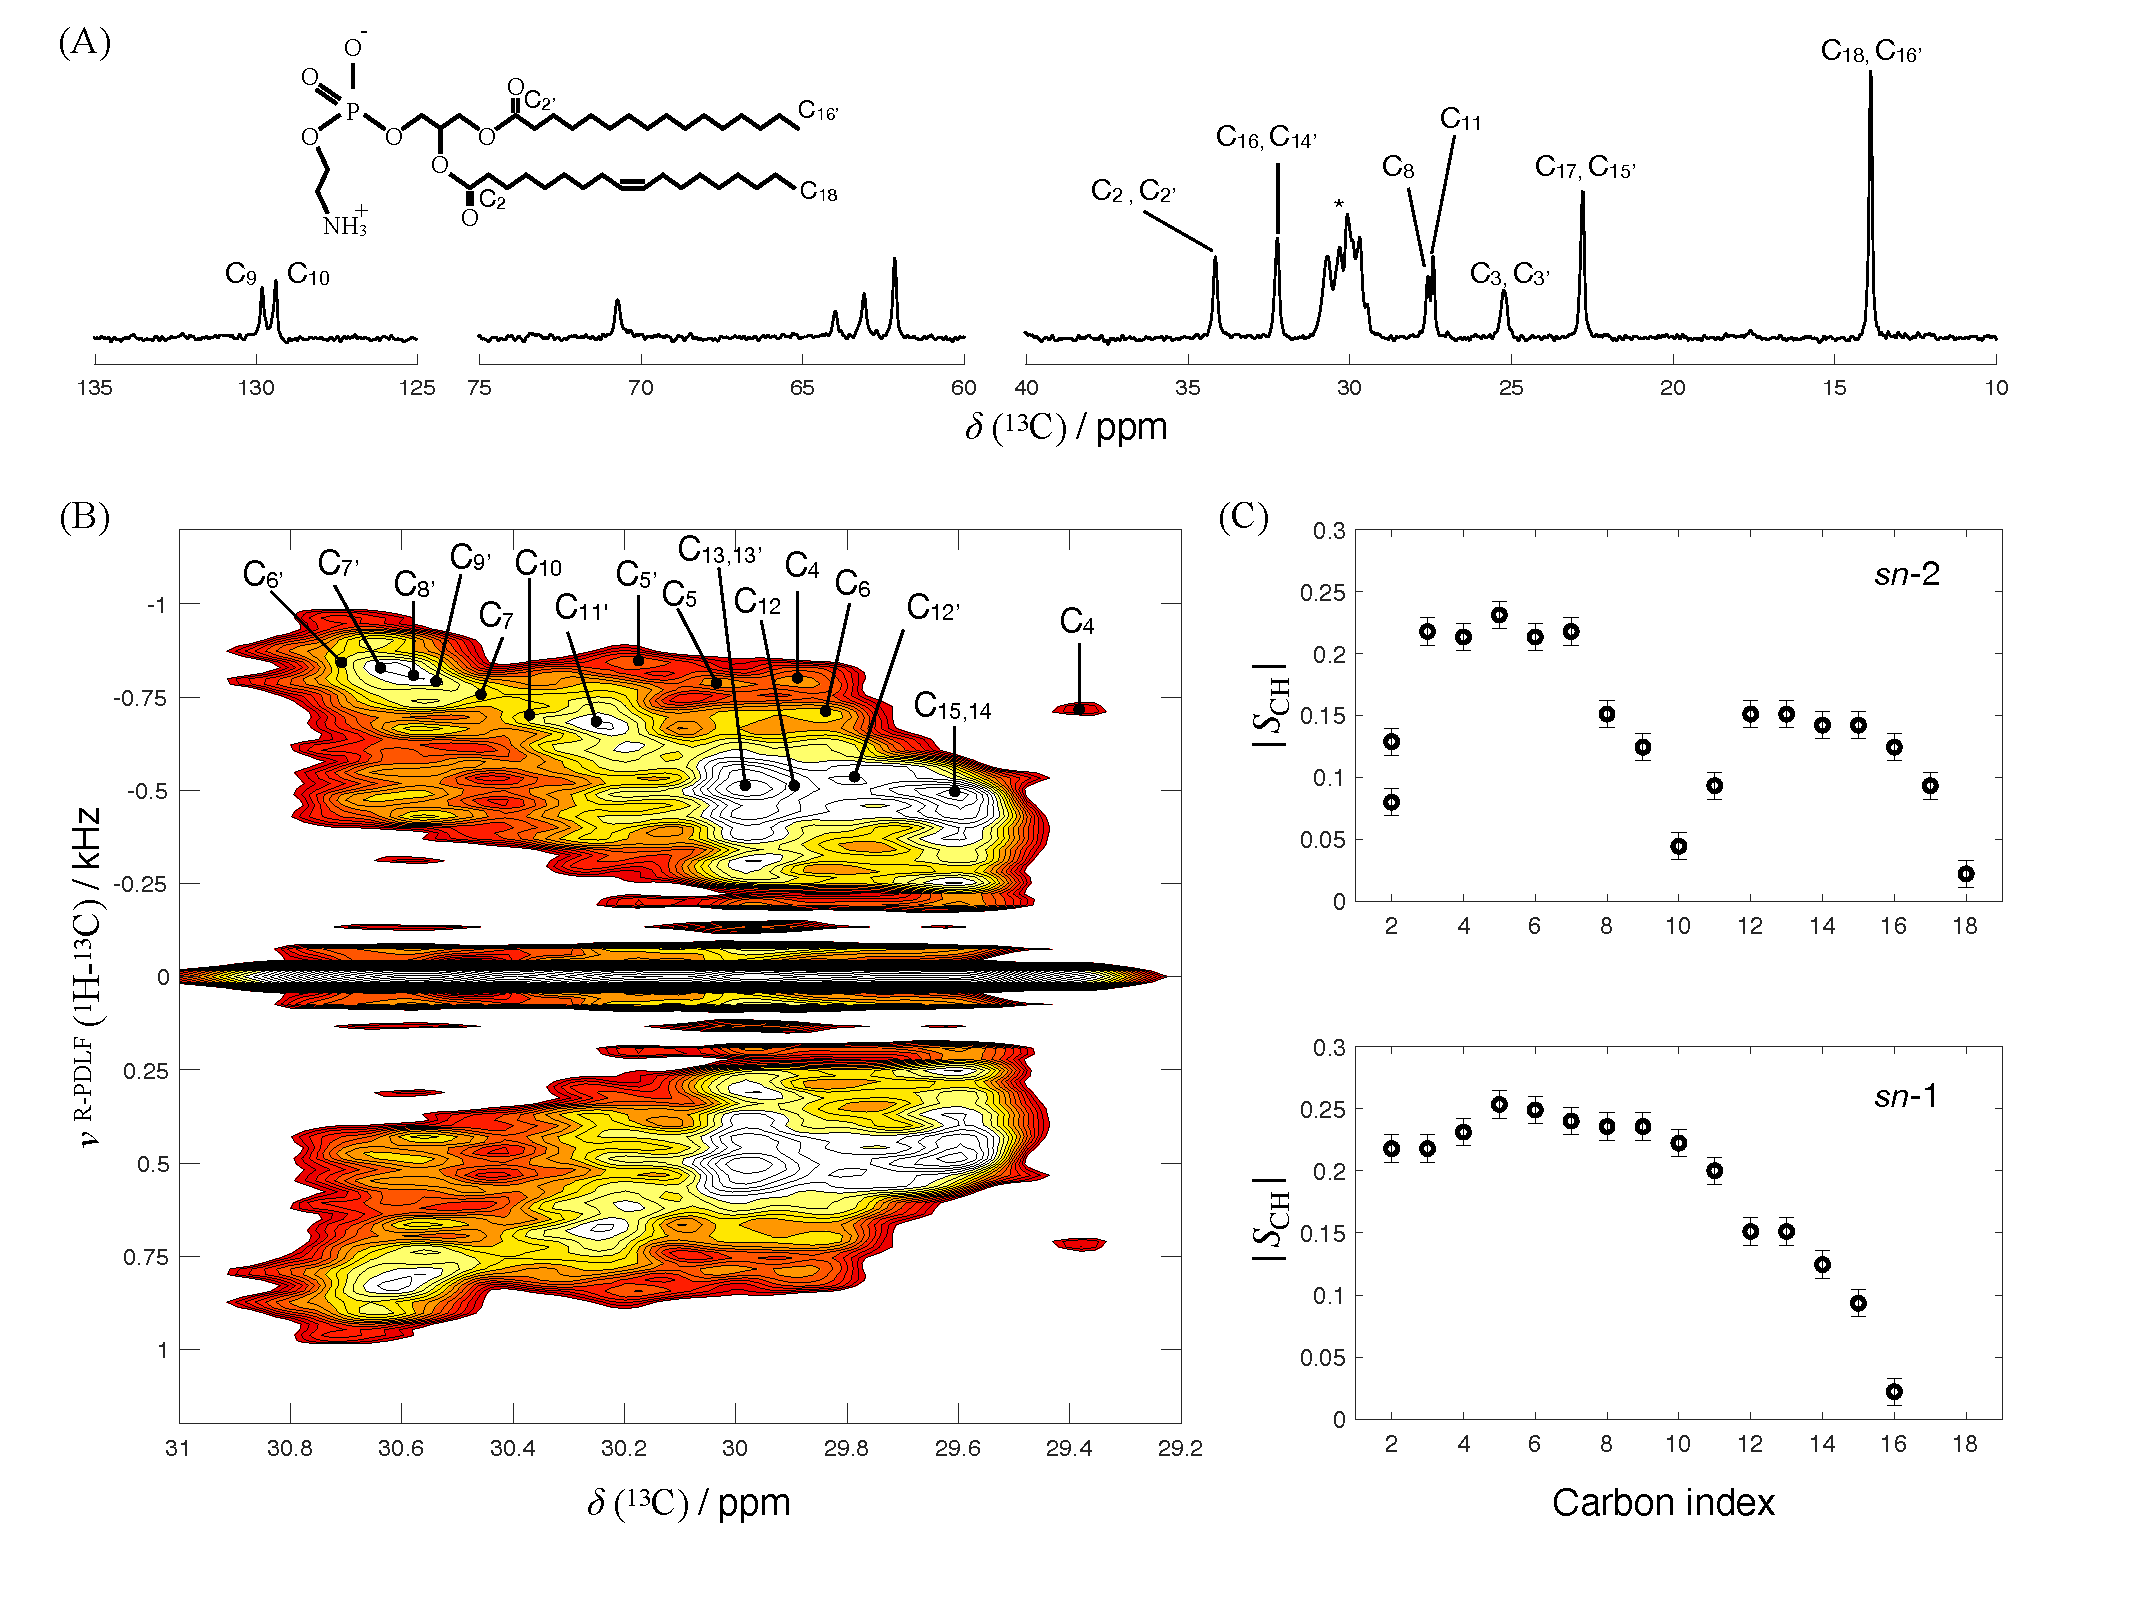
\includegraphics[width=\textwidth]{Figures/POPE_INEPT_contour_SCH.pdf}
  \caption{Determination of the POPE acyl chain order parameters from a R-PDLF spectrum measured at a magic angle spinning frequency of 5.15 kHz. (A) $^{13}$C rINEPT spectrum with peak assignment. The labels used are shown in the chemical structure of POPE. The chemical shift of the methyl groups was defined as 13.8 ppm. (B) Contour plot of the R-PDLF spectrum for the crowded spectral region. The assignment was based on a previous assignment reported for POPC membranes~\cite{ferreira13}. (C) C--H bond order parameter profile for the acyl chains of POPE. The splittings used for calculating the order parameters are shown in Fig.~\ref{POPEexp2}. The unassigned peaks belong to the headgroup and glycerol backbone carbons. A detailed assignment and order parameter analysis of these carbons was shown previously~\cite{bacle21}.      }
  \label{POPEexp1}
\end{figure}

\begin{figure}[p]
  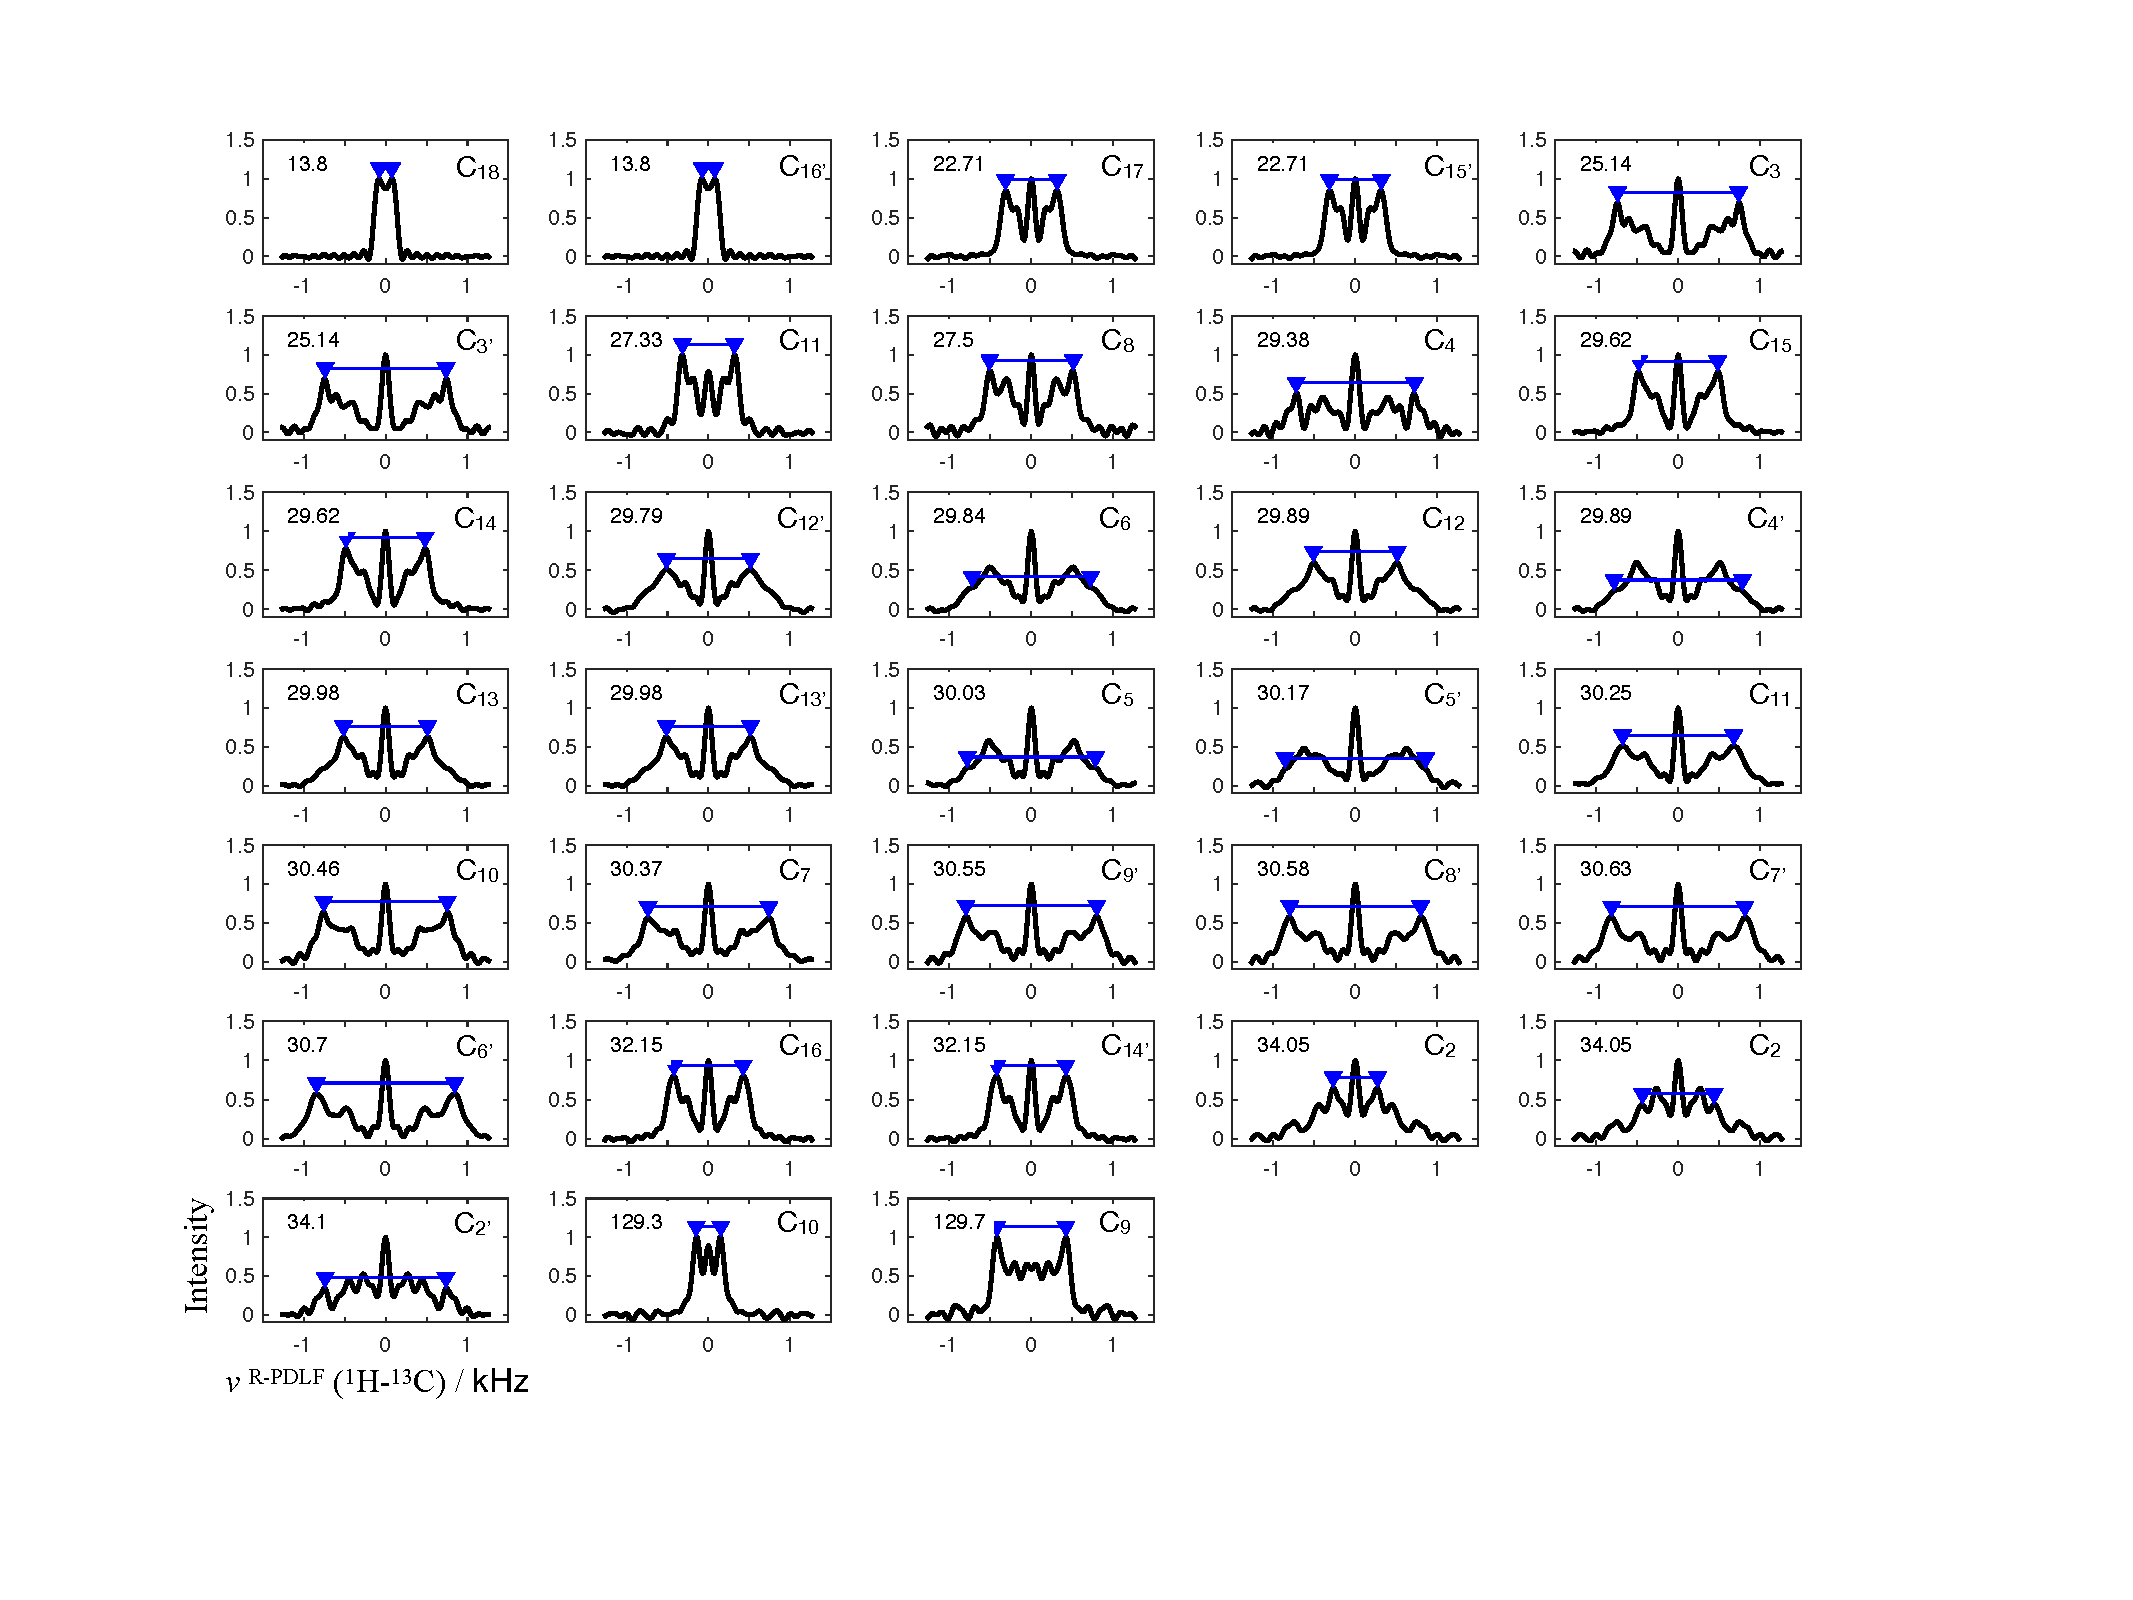
\includegraphics[width=\textwidth]{Figures/POPE_slices.pdf}
  \caption{Dipolar spectra obtained from the 2D R-PDLF spectrum from POPE in Fig.~\ref{POPEexp1}. The number at the top left corner of each panel denotes the corresponding chemical shift. The carbon label for each splitting is displayed on the top right corner. The labels are the same as in Fig.~\ref{POPEexp1}.  }
  \label{POPEexp2}
\end{figure}

\begin{figure}[p]
  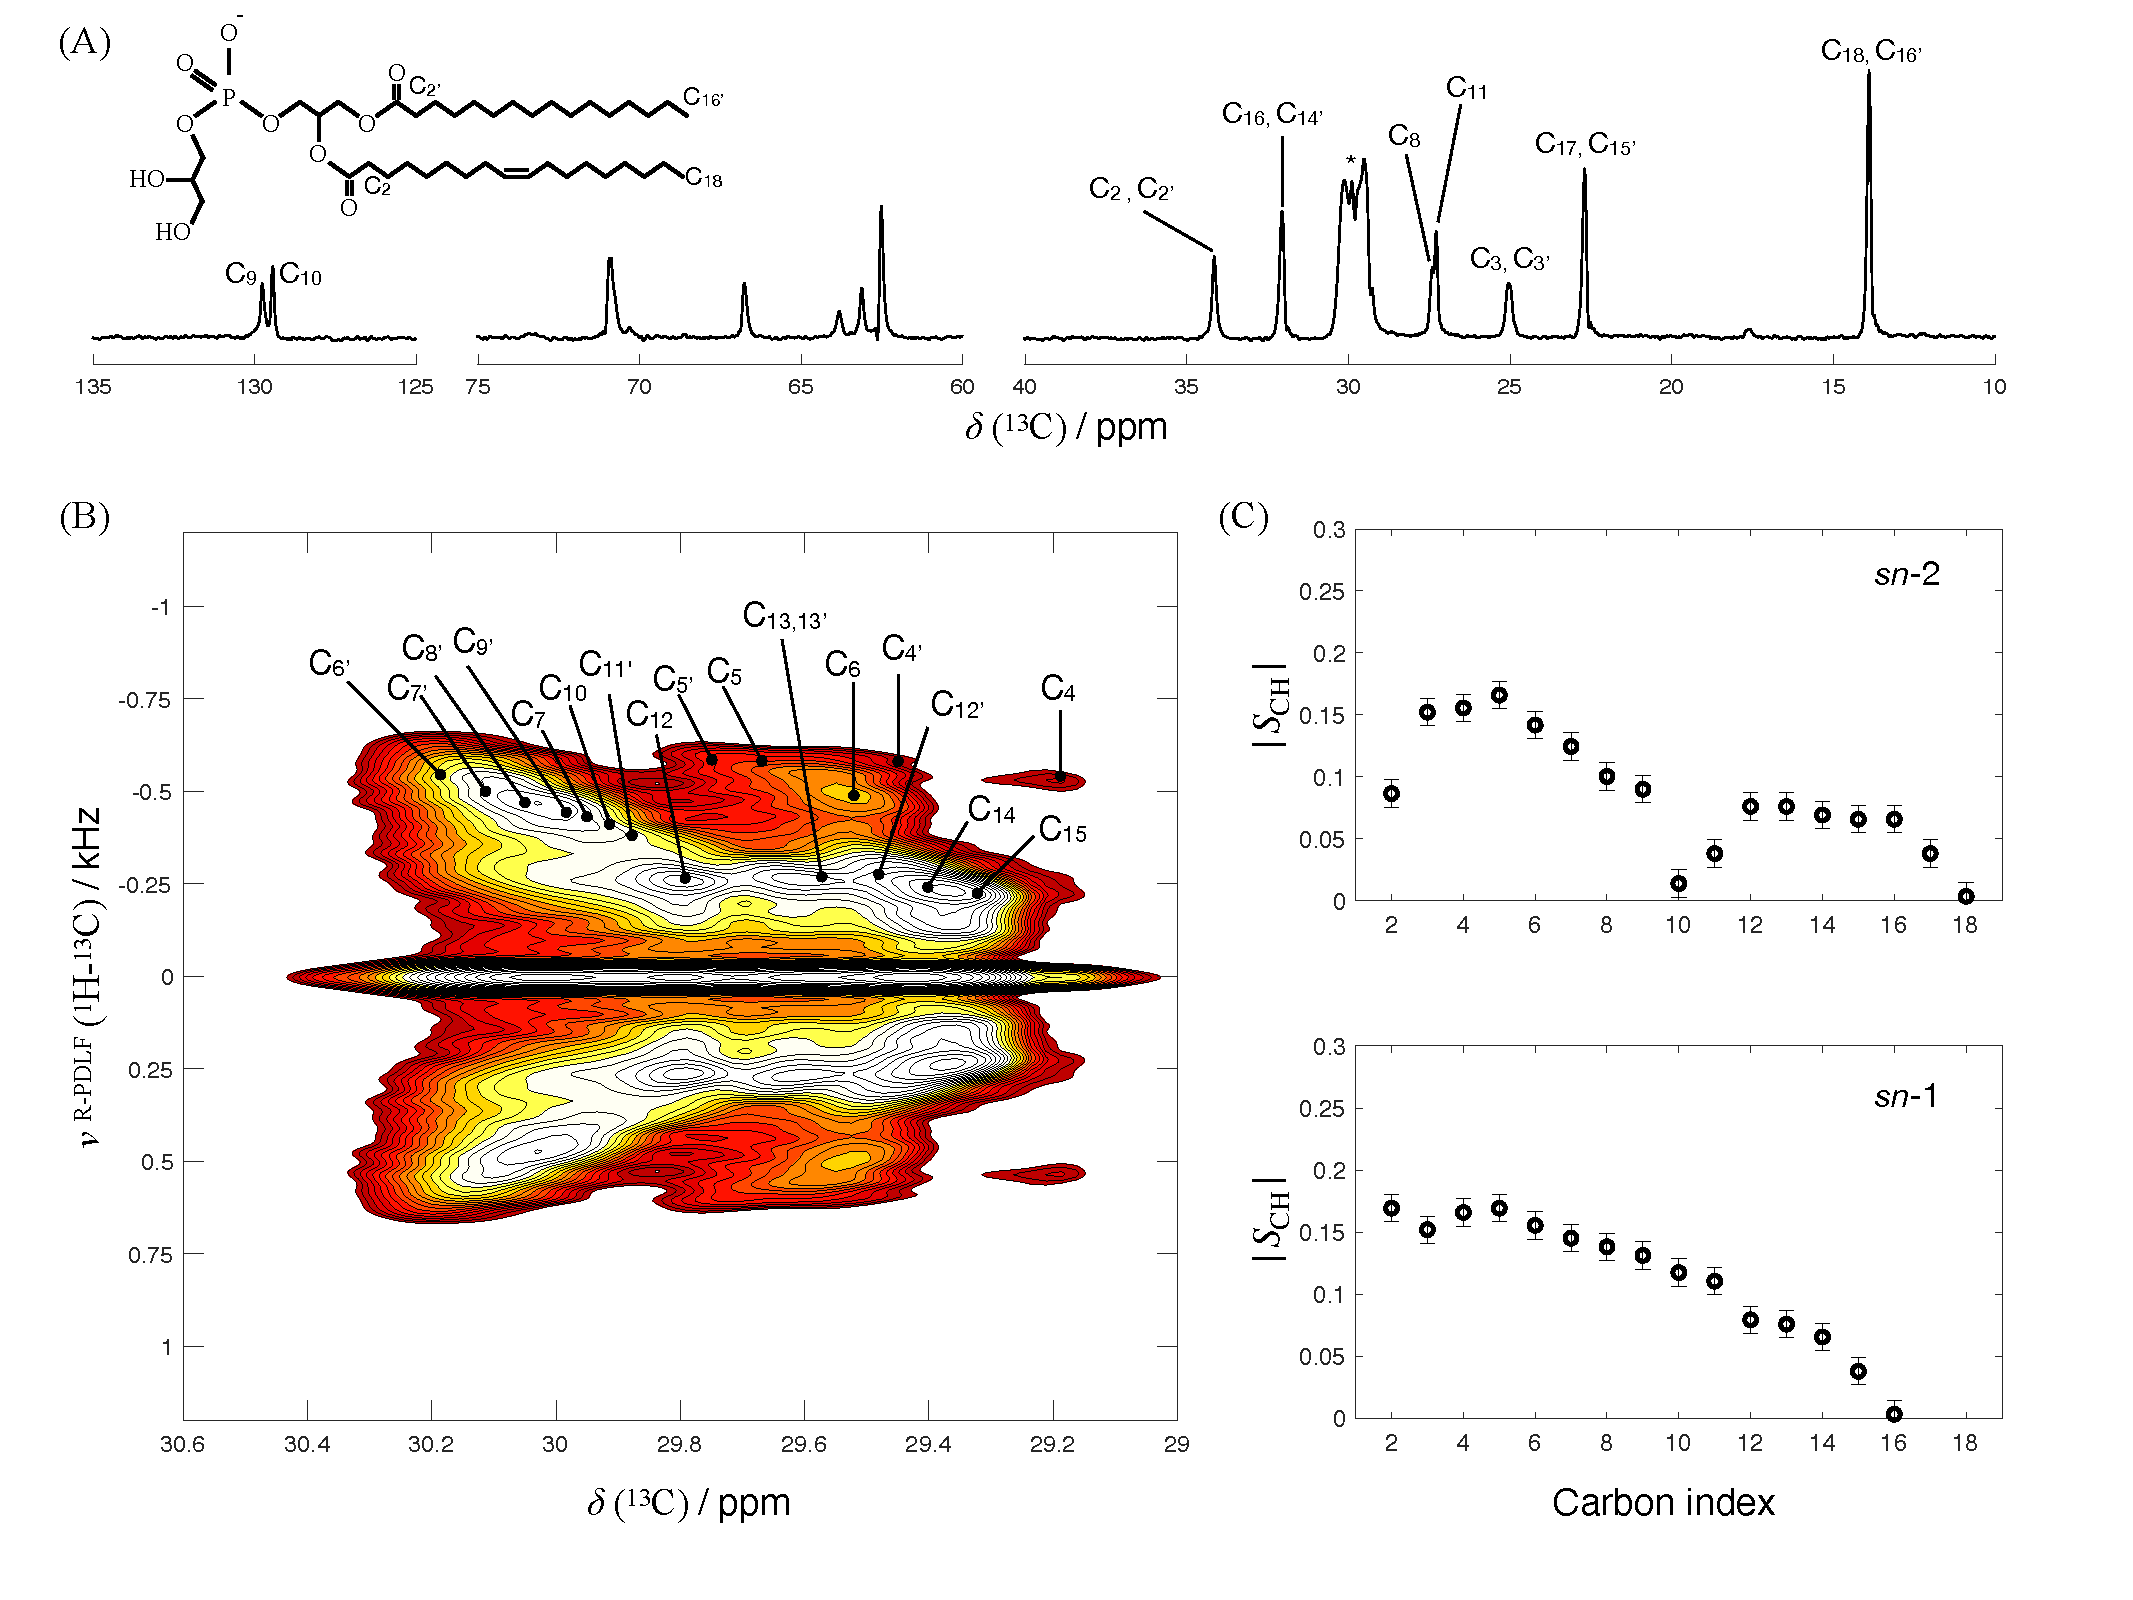
\includegraphics[width=\textwidth]{Figures/POPG_INEPT_contour_SCH.pdf}
  \caption{Determination of the POPG acyl chain order parameters from a R-PDLF spectrum measured at a magic angle spinning frequency of 5.15 kHz. (A) $^{13}$C rINEPT spectrum with peak assignment. The labels used are shown in the chemical structure of POPG. The chemical shift of the methyl groups was defined as 13.8 ppm. (B) Contour plot of the R-PDLF spectrum for the crowded spectral region. The assignment was based on a previous assignment reported for POPC membranes~\cite{ferreira13}. (C) C--H bond order parameter profile for the acyl chains of POPG. The splittings used for calculating the order parameters are shown in Fig.~\ref{POPGexp2}. The unassigned peaks belong to the headgroup and glycerol backbone carbons. A detailed assignment and order parameter analysis of these carbons was shown previously~\cite{bacle21}.}
  \label{POPGexp1}
\end{figure}

\begin{figure}[p]
  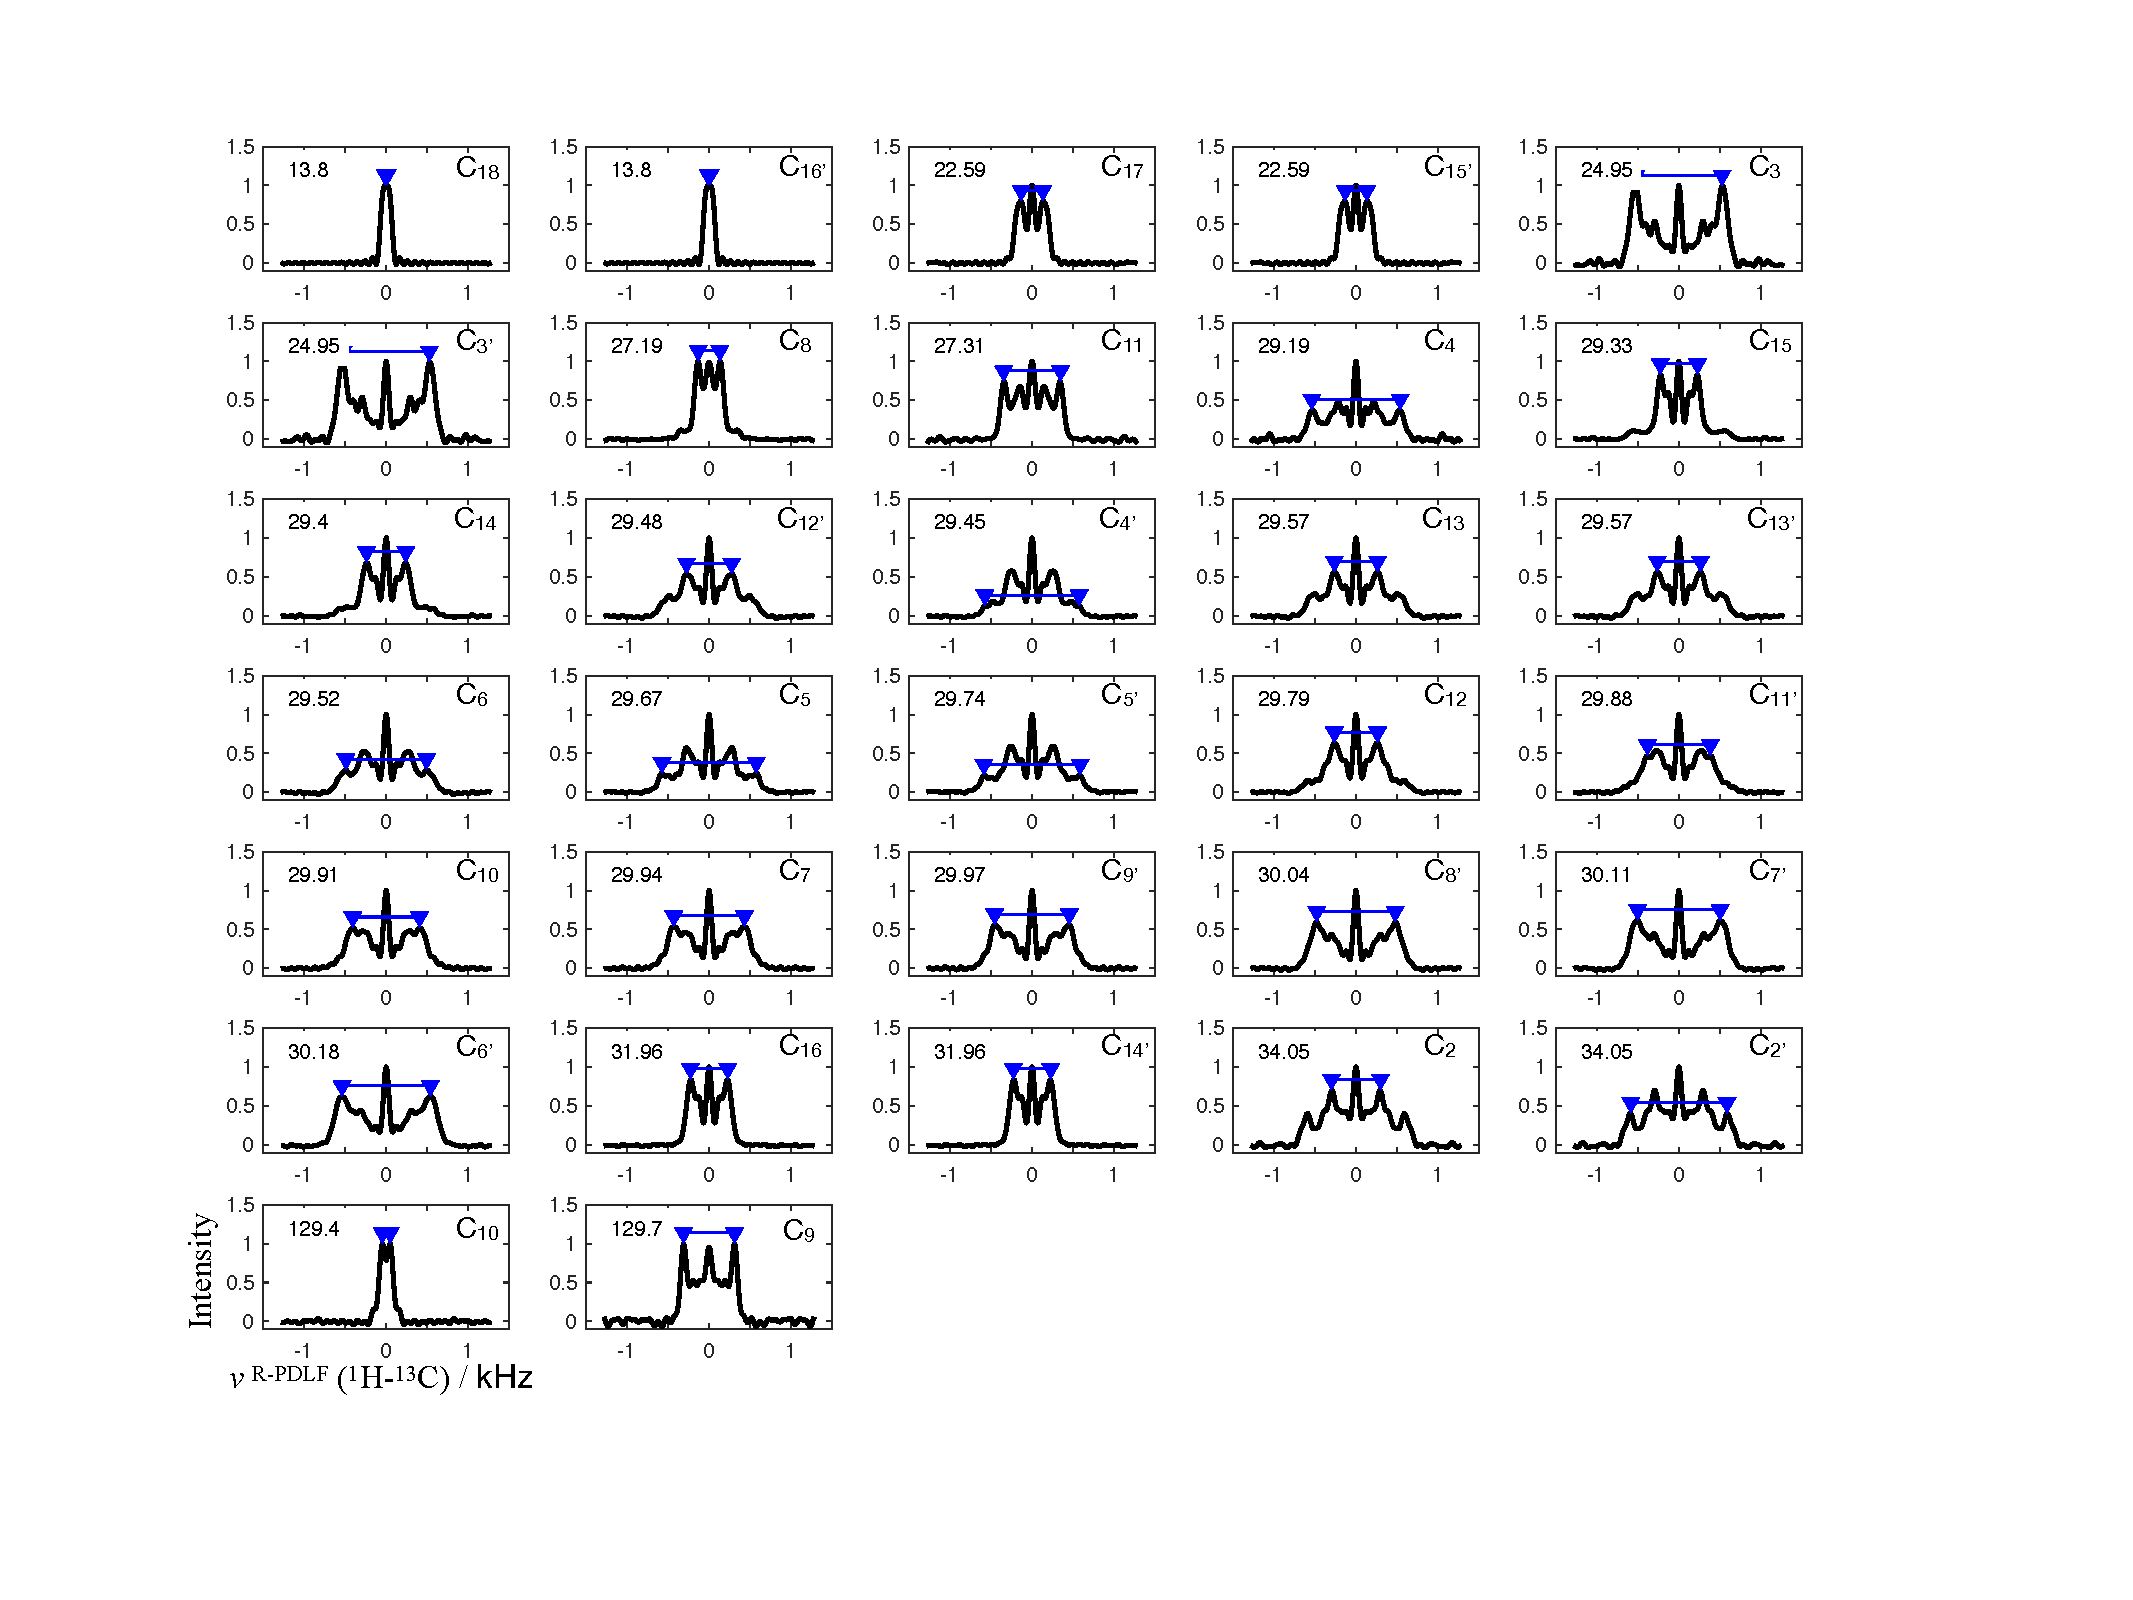
\includegraphics[width=\textwidth]{Figures/POPG_slices.pdf}
  \caption{Dipolar spectra obtained from the 2D R-PDLF spectrum described in Fig.~\ref{POPGexp1}. The number at the top left corner of each panel denotes the corresponding chemical shift. The carbon label for each splitting is displayed on the top right corner. The labels are the same as in Fig.~\ref{POPGexp1}. }
  \label{POPGexp2}
\end{figure}

\begin{figure}
    \centering
    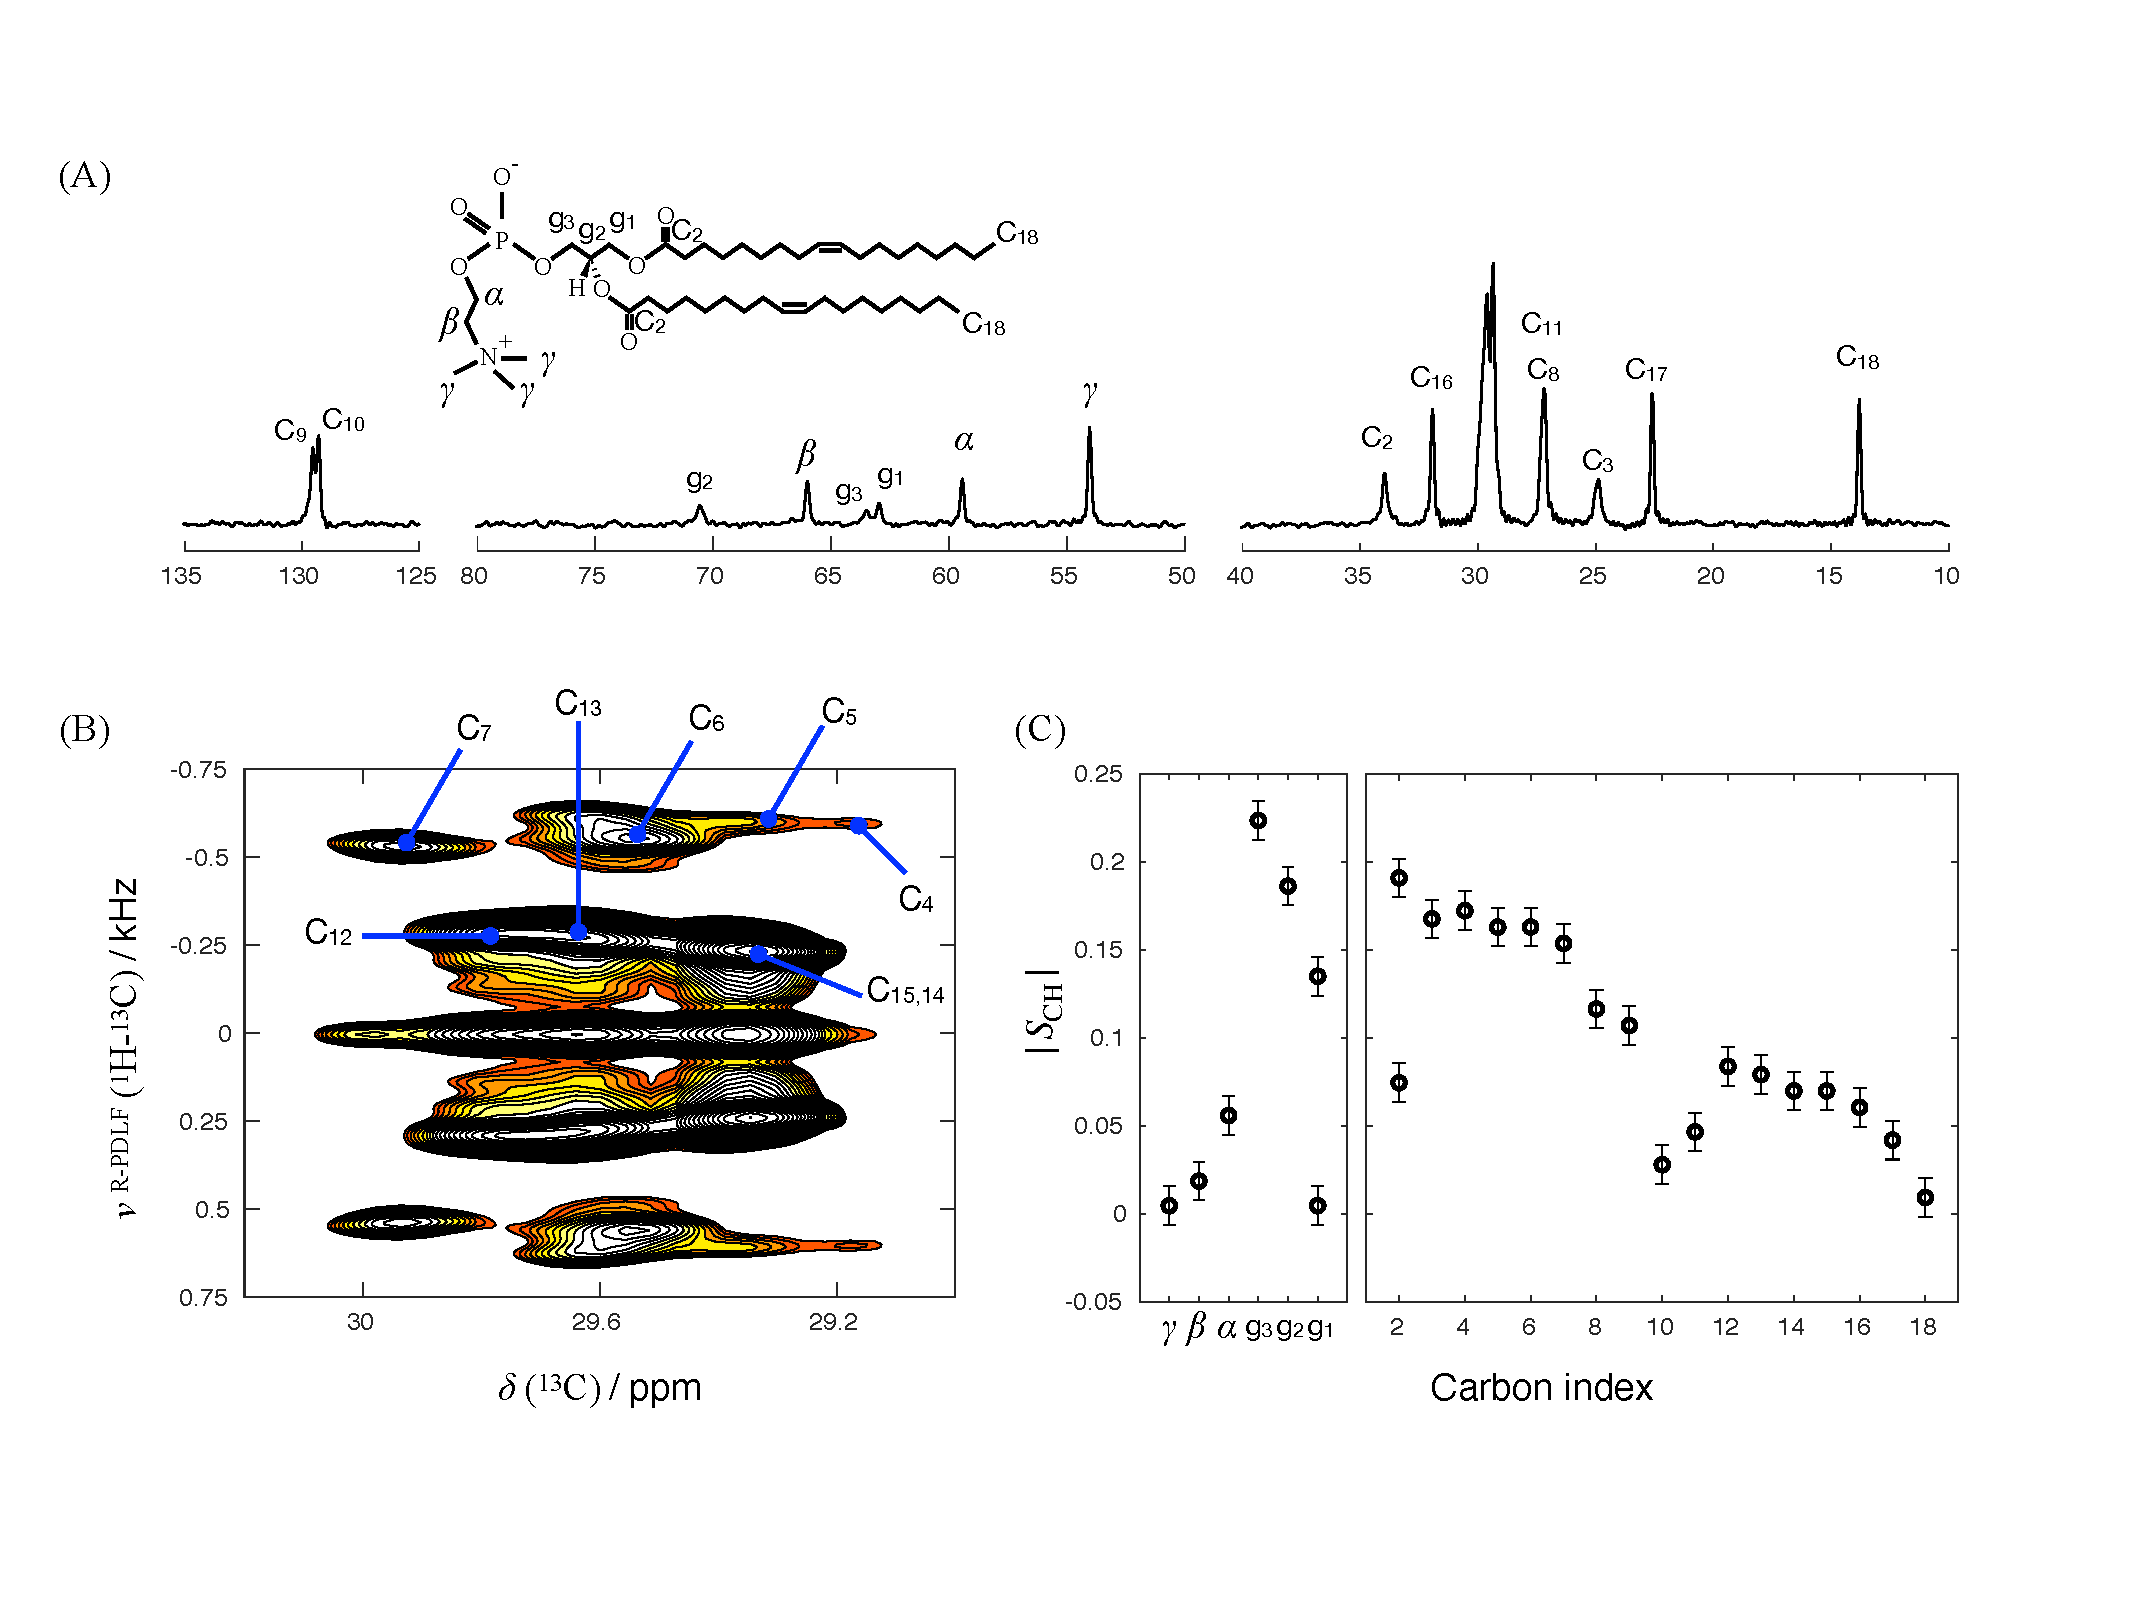
\includegraphics[width=\textwidth]{Figures/DOPCfig.pdf}
    \caption{Determination of DOPC order parameters from a R-PDLF spectrum measured at a magic angle spinning frequency of 5.15 kHz. (A) $^{13}$C rINEPT spectrum with peak assignment. The labels used are shown in the chemical structure of DOPC. The chemical shift of the methyl groups was defined as 13.8 ppm. (B) Contour plot of the R-PDLF spectrum for the crowded spectral region. The assignment was based on a previous assignment reported for POPC membranes~\cite{ferreira13}. (C) C--H bond order parameters of DOPC.}
    \label{fig:DOPCexp}
\end{figure}

\begin{figure}[p]
  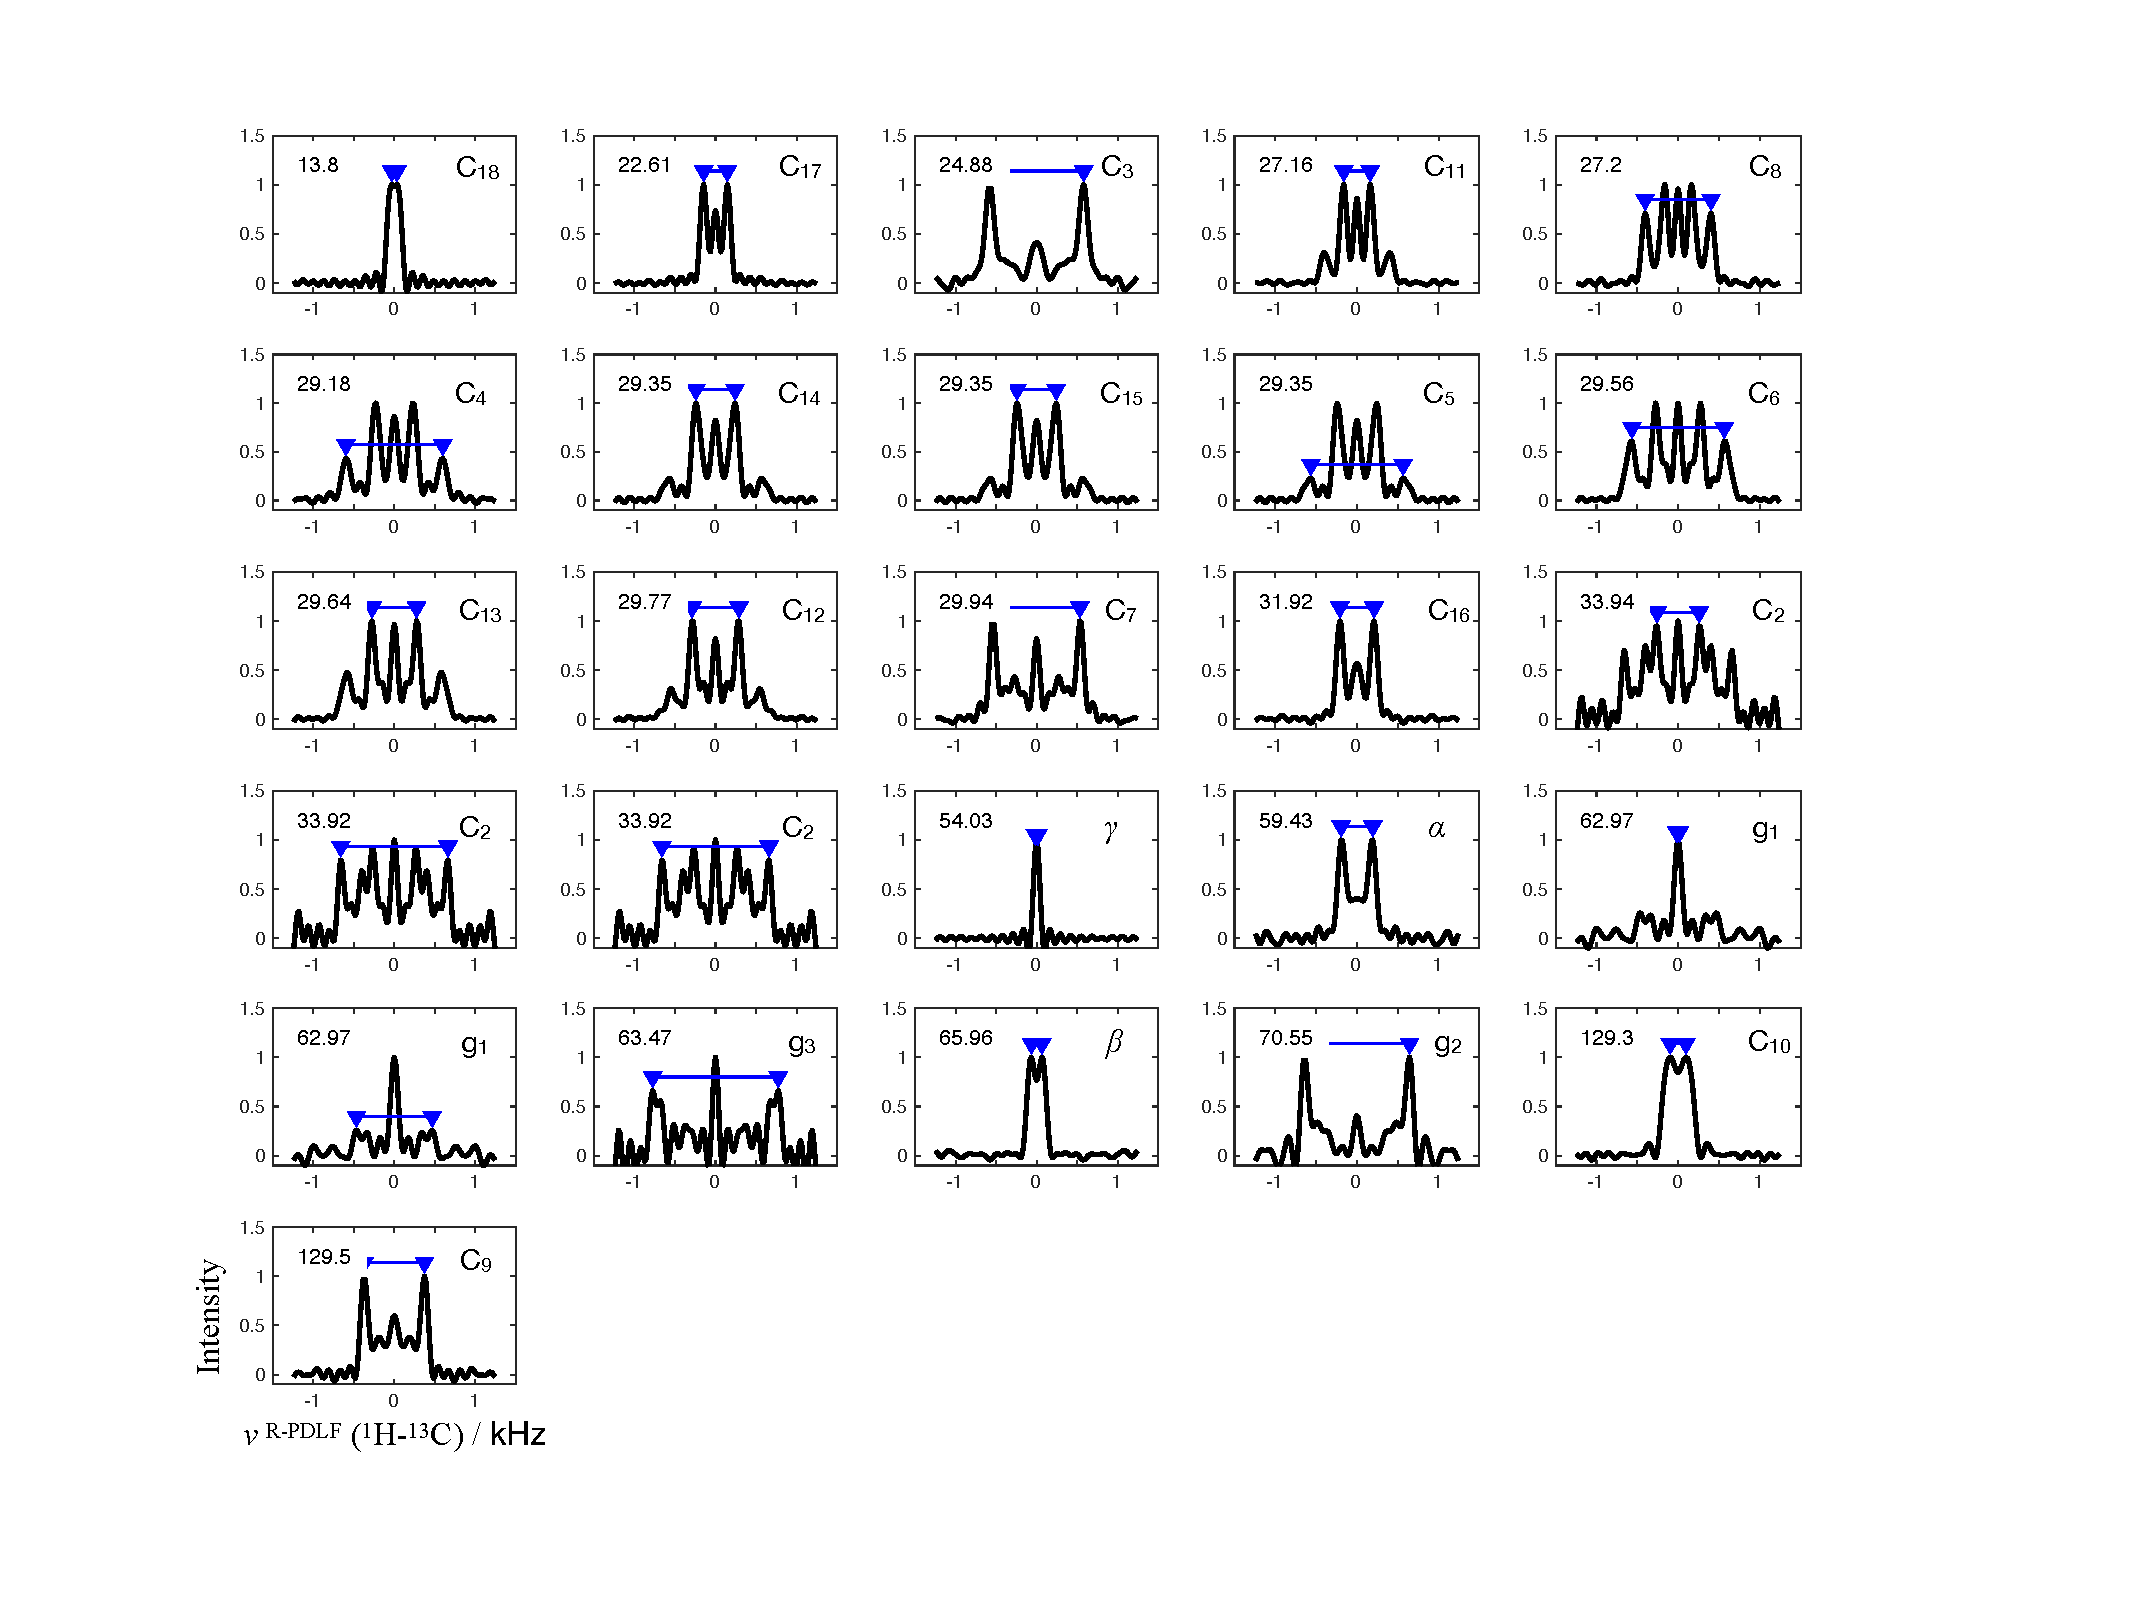
\includegraphics[width=\textwidth]{Figures/DOPC_slices.pdf}
  \caption{Dipolar spectra obtained from the 2D R-PDLF spectrum described in Fig.~\ref{fig:DOPCexp}. The number at the top left corner of each panel denotes the corresponding chemical shift. The carbon label for each splitting is displayed on the top right corner. The labels are the same as in Fig.~\ref{fig:DOPCexp}. }
  \label{DOPCexp2}
\end{figure}



%\pagebreak
%\subsection{X-ray scattering experiments}
%X-ray scattering form factors contributed to the NMRlipids III project are included in the databank (\url{http://nmrlipids.blogspot.com/2022/09/nmrlipids-iii-including-lipid-lateral.html}).


\pagebreak
\bibliography{refs.bib}

%\noindent LaTeX formats citations and references automatically using the bibliography records in your .bib file, which you can edit via the project menu. Use the cite command for an inline citation, e.g.  \cite{Hao:gidmaps:2014}.

%For data citations of datasets uploaded to e.g. \emph{figshare}, please use the \verb|howpublished| option in the bib entry to specify the platform and the link, as in the \verb|Hao:gidmaps:2014| example in the sample bibliography file.

%\section*{Acknowledgements}

%Acknowledgements should be brief, and should not include thanks to anonymous referees and editors, or effusive comments. Grant or contribution numbers may be acknowledged.

%\section*{Author contributions statement}

%Must include all authors, identified by initials, for example:
%A.A. conceived the experiment(s),  A.A. and B.A. conducted the experiment(s), C.A. and D.A. analysed the results.  All authors reviewed the manuscript. 

%\section*{Additional information}

%To include, in this order: \textbf{Accession codes} (where applicable); \textbf{Competing interests} (mandatory statement). 

%The corresponding author is responsible for submitting a \href{http://www.nature.com/srep/policies/index.html#competing}{competing interests statement} on behalf of all authors of the paper. This statement must be included in the submitted article file.

%\begin{figure}[ht]
%\centering
%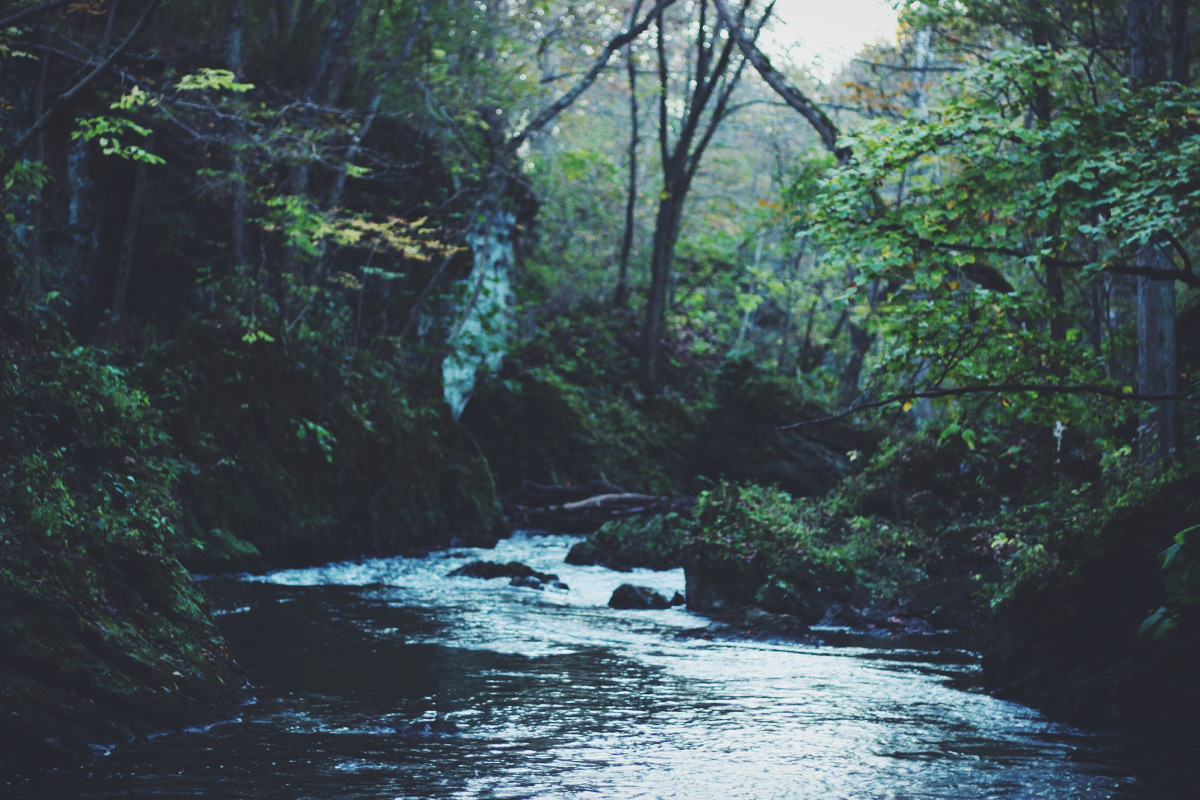
\includegraphics[width=\linewidth]{stream}
%%\caption{Legend (350 words max). Example legend text.}
%\label{fig:stream}
%\end{figure}

%\begin{table}[ht]
%\centering
%\begin{tabular}{|l|l|l|}
%\hline
%Condition & n & p \\
%\hline
%A & 5 & 0.1 \\
%\hline
%B & 10 & 0.01 \\
%\hline
%\end{tabular}
%\caption{\label{tab:example}Legend (350 words max). Example legend text.}
%\end{table}

%Figures and tables can be referenced in LaTeX using the ref command, e.g. Figure \ref{fig:stream} and Table \ref{tab:example}.

\end{document}
